% Chapter 2

\chapter{\normf{理论基础}}
本文所研究的多传感器标定算法是一种基于自运动的时空参数标定方法,其基于连续时间理论,通过因子图优化的方式估计待标参数。因此,在介绍算法之前,有必要进行相关理论的阐述和相关符号的说明。

\section{\normf{坐标系定义}}
本文提出的标定方法涉及内参、外参和时参,其中描述不同传感器坐标系之间相对位姿关系的外参是较为重要的一部分,其涉及到了传感器坐标系的表示。本文所研究的算法涉及LiDAR、Camera和IMU这三种传感器,下面依次给出各传感器坐标系的定义。
\begin{enumerate}
  \item LiDAR坐标系

        LiDAR坐标系以激光脉冲发射中心作为原点,其Y轴指向正前方,Z轴指向天顶方向,X轴与Y轴和Z轴构成右手直角坐标系。本文用字母$L$表示LiDAR坐标系,用花体字母$\mathcal{L}$表示LiDAR坐标系序列,用$L_i$表示序列中的第$i$个LiDAR坐标系,其中$i\in\mathcal{L}^\dagger$。符号$(\cdot)^\dagger$表示对序列集合元素取标号的操作。
  \item Camera坐标系

        Camera坐标系以相机光心作为原点,其Z轴指向正前方(即相机主光轴方向),X轴垂直于Z轴向右,Y轴与X轴和Z轴构成右手直角坐标系,指向天顶方向的反方向。本文用字母$C$表示Camera坐标系,用花体字母$\mathcal{C}$表示Camera坐标系序列,用$C_j$表示序列中的第$j$个Camera坐标系,其中$j\in\mathcal{C}^\dagger$。
  \item IMU坐标系

        IMU是由加速度计和陀螺仪两种器件构成,安装时二者的坐标系可能不一致\footnote{\normf{该偏差被称为IMU安装误差(IMU Misalignment)。在本标定算法中会考虑这个偏差,详细内容见\ref{sensro_model_imu}节。}}。在本文中,将加速度计坐标系视为IMU坐标系,即在加速度计不存在交轴耦合误差\footnote{\normf{指三个轴不严格正交,详细内容见\ref{sensro_model_imu}节。}}(Axis Misalignment)的前提下,IMU坐标系的三个正交轴和加速度计坐标系的轴向完全重合。IMU坐标系也是一个右手直角坐标系,本文用字母$I$表示该坐标系,用字母$A$、$G$表示加速度计和陀螺仪的坐标系,用花体字母$\mathcal{I}$表示IMU坐标系序列,用$I_k$表示序列中的第$k$个IMU坐标系,其中$k\in\mathcal{I}^\dagger$。
\end{enumerate}
\section{\normf{坐标系刚体变换}}
三维刚体变换(Rigid Body Transformation)描述了三维空间中两个刚体坐标系之间的相对位姿关系,其由姿态量和平移量构成,存在6个自由度,具有多种数学表达形式。下面对常用的几种表达形式进行阐述。
\subsection{\normf{变换矩阵}}
变换矩阵(Transform Matrix)由旋转矩阵和平移向量构成,通过下式定义:
\begin{equation}
  \boldsymbol{T}=\begin{pmatrix}
    \boldsymbol{R} & \boldsymbol{p} \\\boldsymbol{0}&1
  \end{pmatrix}\in\mathrm{SE(3)}\quad \mathrm{s.t.}\quad\boldsymbol{R}\in \mathrm{SO(3)},\;\boldsymbol{p}\in \mathbb{R}^3
\end{equation}
其中:$\boldsymbol{R}$为旋转矩阵,其存在于三维空间中的特殊正交群SO(3)中,同时也是一个单位正交阵\footnote{\normf{即旋转矩阵满足$\boldsymbol{R}\boldsymbol{R}^T=\boldsymbol{I},\det\boldsymbol{R}=1$。}};$\boldsymbol{p}$是三维的平移向量;$\boldsymbol{T}$即为变换矩阵,其存在于三维空间中的特殊欧式群SE(3)中。对于自由度为6的三维刚体变换而言,变换矩阵是冗余的,不是最小表达形式。
\subsection{\normf{欧拉角和轴角}}
欧拉角(Euler Angles)使用三个绕正交轴旋转的角来表示姿态,结合平移向量,同样可以表达三维刚体变换。对于一次刚体旋转,可以将其分解为三次绕轴旋转的角,相应的,也可以通过依次绕指定轴旋转相应的角度恢复出刚体旋转。欧拉角与绕轴旋转的顺序相关,顺序不同,结果也会不同。其中最为常用的是“翻滚-俯仰-航偏”(roll-pitch-yaw)的欧拉角,即rpy角。欧拉角是三维刚体旋转的最小表达形式,且较为直观,但存在万向锁问题(Gimbal Lock),会导致旋转奇异。如对于rpy角而言,当俯仰角为$\pm \pi/2$时,翻滚角和航偏角绕空间中的同一个轴旋转,导致一个自由度的丢失。

另外,刚体旋转也可以直接表示为绕空间某个轴旋转一个角的形式,该种表达形式被称为轴角(Axis Angle)或者旋转向量。轴角一般用向量$\boldsymbol{\theta}\in\mathbb{R}^3$表示,向量的指向即为旋转轴的方向,向量的模长即为旋转角度的大小。轴角同样也是三维刚体旋转的最小表达形式。

\subsection{\normf{单位四元数}}
单位四元数(Unit Quaternion)用一个实数和三个虚数构成的四维单位向量表示旋转,相比欧拉角多了一个自由度\footnote{\normf{相对应的,也多了一个约束,即模长为单位1。}},但是不存在奇异问题,是一种紧凑的表达形式。单位四元数的定义如下:
\begin{equation}
  \boldsymbol{q}=q_w+q_x\boldsymbol{i}+q_y\boldsymbol{j}+q_z\boldsymbol{k}\quad \mathrm{s.t.}\quad
  \begin{cases}
    \boldsymbol{i}^2=\boldsymbol{j}^2=\boldsymbol{k}^2=-1                                                                                       \\
    \boldsymbol{i}\boldsymbol{j}=\boldsymbol{k}\quad\boldsymbol{j}\boldsymbol{k}=\boldsymbol{i}\quad\boldsymbol{k}\boldsymbol{i}=\boldsymbol{j} \\
    q_w^2+q_x^2+q_y^2+q_z^2=1^2
  \end{cases}
\end{equation}
其中$\boldsymbol{i}$、$\boldsymbol{j}$、$\boldsymbol{k}$为虚数单位。单位四元数可以表示成显含轴角的形式:
\begin{equation}
  \boldsymbol{q}=\cos\frac{\Vert \boldsymbol{\theta}\Vert}{2}+\frac{\boldsymbol{\theta}}{\Vert \boldsymbol{\theta}\Vert}\sin\frac{\Vert \boldsymbol{\theta}\Vert}{2}
\end{equation}
\subsection{\normf{李代数}}
三维刚体变换的另一种最小表示是李代数(Lie Algebra)。与旋转矩阵$\boldsymbol{R}$在流形(Manifold)上表示旋转不同,姿态李代数$\boldsymbol{\liehat{\boldsymbol{\phi}}}\in\mathfrak{so}(3)$在正切空间(Tangent Space)表示旋转,因此当涉及优化问题中的雅克比矩阵求解和状态增量更新时较为简洁便利(具体见附录\ref{appendix:lie_alg_update})。其中$\liehat{\cdot}$表示将三维向量映射为反对称矩阵,与此对应的$\lievee{\cdot}$则将反对称矩阵映射为三维向量,即:
\begin{equation}
  \boldsymbol{\phi}=\begin{pmatrix}
    \phi_x \\\phi_y\\\phi_z
  \end{pmatrix}\in\mathbb{R}^3 \quad
  \liehat{\boldsymbol{\phi}}=\begin{pmatrix}
    0       & -\phi_z & \phi_y  \\
    \phi_z  & 0       & -\phi_x \\
    -\phi_y & \phi_x  & 0       \\
  \end{pmatrix}\quad \liehatvee{\boldsymbol{\phi}}=\boldsymbol{\phi}
\end{equation}

姿态李代数$\boldsymbol{\liehat{\boldsymbol{\phi}}}$和旋转矩阵$\boldsymbol{R}$之间的转换可以通过指数映射和对数映射实现:
\begin{equation}
  \boldsymbol{R}=\exp(\liehat{\boldsymbol{\phi}}) \quad \liehat{\boldsymbol{\phi}}=\log(\boldsymbol{R})
\end{equation}
而首字母大写的指数映射和对数映射,则可直接建立姿态李代数向量$\boldsymbol{\phi}$和旋转矩阵$\boldsymbol{R}$之间的关系:
\begin{equation}
  \boldsymbol{R}=\mathrm{Exp}(\boldsymbol{\phi}) \quad \boldsymbol{\phi}=\mathrm{Log}(\boldsymbol{R})
\end{equation}
除了可以建立SO(3)和$\mathfrak{so}(3)$之间的映射外,还存在SE(3)和$\mathfrak{se}(3)$之间的映射,后者使用6维向量同时表达姿态量和位移量,这里不再介绍,具体可参考\cite{sola2018micro}。

\subsection{\normf{坐标系变换}}
假设空间中存在两个坐标系$F_i$、$F_j$,以及点$\boldsymbol{p}$和向量$\boldsymbol{v}$,则将点或向量从$F_i$系变换到$F_j$系的过程,可以等价表达为如表\ref{tab:rbt}所示的不同形式。
\begin{table*}[htbp]
  \centering
  \caption{\normf{点和向量坐标系变换的不同表达形式}}
  \label{tab:rbt}
  \begin{tabular}{c|c|c|c|c}
    \hline
    \normf{对象}             & \normf{${^{j}_{i}}\boldsymbol{T}$}                          & \normf{${^{j}_{i}}\boldsymbol{R}$和${^{j}\boldsymbol{p}_{i}}$} & \normf{${^{j}_{i}}\boldsymbol{q}$和${^{j}\boldsymbol{p}_{i}}$} & \normf{${^{j}_{i}}\boldsymbol{\phi}$和${^{j}\boldsymbol{p}_{i}}$} \\ \hline
                             &                                                             &                                                                &                                                                &                                                                   \\
    \normf{$\boldsymbol{p}$} & $\begin{pmatrix}
                                    {^{j}}\boldsymbol{p} \\1
                                  \end{pmatrix}={^{j}_{i}}\boldsymbol{T} \circ\begin{pmatrix}
                                                                                {^{i}}\boldsymbol{p} \\1
                                                                              \end{pmatrix}$
                             &
    ${^{j}}\boldsymbol{p}={^{\boldsymbol{j}}_{\boldsymbol{i}}}\boldsymbol{R}\circ{^{i}}\boldsymbol{p}+{^{j}\boldsymbol{p}_{i}}$
                             &
    ${^{j}}\boldsymbol{p}={^{\boldsymbol{j}}_{\boldsymbol{i}}}\boldsymbol{q}\circ{^{i}}\boldsymbol{p}+{^{j}\boldsymbol{p}_{i}}$
                             &
    ${^{j}}\boldsymbol{p}={^{\boldsymbol{j}}_{\boldsymbol{i}}}\boldsymbol{\phi}\circ{^{i}}\boldsymbol{p}+{^{j}\boldsymbol{p}_{i}}$                                                                                                                                                               \\ &&&&\\
    \normf{$\boldsymbol{v}$}
                             &
    $\begin{pmatrix}
         {^{j}}\boldsymbol{v} \\0
       \end{pmatrix}={^{j}_{i}}\boldsymbol{T} \circ\begin{pmatrix}
                                                     {^{i}}\boldsymbol{v} \\0
                                                   \end{pmatrix}$
                             &
    ${^{j}}\boldsymbol{v}={^{\boldsymbol{j}}_{\boldsymbol{i}}}\boldsymbol{R}\circ{^{i}}\boldsymbol{v}$
                             &
    ${^{j}}\boldsymbol{v}={^{\boldsymbol{j}}_{\boldsymbol{i}}}\boldsymbol{q}\circ{^{i}}\boldsymbol{v}$
                             &
    ${^{j}}\boldsymbol{v}={^{\boldsymbol{j}}_{\boldsymbol{i}}}\boldsymbol{\phi}\circ{^{i}}\boldsymbol{v}$                                                                                                                                                                                        \\
                             &                                                             &                                                                &                                                                &                                                                   \\
    \hline
  \end{tabular}
\end{table*}
\newline
其中:$\circ$表示相应的群运算、代数运算或矩阵运算,具体可参考文献\cite{sola2018micro};${^{i\mid j}}(\boldsymbol{p}\mid\boldsymbol{v})$表示点或向量在参考坐标系$F_{i\mid j}$系下的坐标表达。注意到,对于向量而言,变换坐标系只需考虑旋转量即可。在下文涉及坐标变换时,认为以上几种表达方式是等价的,且省略符号$\circ$的书写,不再具体说明。

\section{\normf{传感器模型及待标参数}}
本文所研究的算法涉及到了LiDAR、Camera和IMU这三种传感器,下面对各传感器模型进行阐述,并基于传感器模型给出本文标定算法框架中的待标参数。
\subsection{\normf{LiDAR}}
激光雷达(Light Detection and Ranging,LiDAR)向目标发射激光光束并接收回波信号,通过信号处理获取目标的相关信息,如距离,方位、反射率等,是一种外部传感器。激光雷达具有分辨率高、体积小、精度高等优点,被广泛应用于智能测绘、自动驾驶等领域。根据扫描方式的不同,激光雷达可分为机械式、固态式和混合固态式三种。由于本文研究的算法主要针对机械式激光雷达,故下面对其进行介绍。

机械式激光雷达在垂向上排布多个激光发射器(Laser Rangerfinder),在数据采集时通过不断地旋转发射器,实现三维场景的扫描。对于空间中探测到的一目标点$\boldsymbol{p}$,基于探测到的距离信息和激光光束的方向信息,可以得到该点在当前$L$系下的三维位置:
\begin{equation}
  \label{equ:lidar_model}
  {^{L}\boldsymbol{p}}=\begin{pmatrix}
    p_x \\
    p_y \\
    p_z
  \end{pmatrix}=\begin{pmatrix}
    d\times\cos\alpha\times\cos\beta \\
    d\times\cos\alpha\times\sin\beta \\
    d\times\sin\alpha
  \end{pmatrix}
\end{equation}
其中:$d$是$L$系坐标原点到点$\boldsymbol{p}$的直线距离,$\alpha$、$\beta$分别是激光光束在扫描点$\boldsymbol{p}$时的旋转角和高度角,如图\ref{fig:lidar_model}所示;${^{L}\boldsymbol{p}}$为点$\boldsymbol{p}$在当前$L$系下的坐标表达。机械式激光雷达发射器旋转一周,采集到的点的集合就构成一帧点云。如果机械式激光雷达采集数据时伴随有运动,则点云帧会存在运动畸变\footnote{\normf{因为在同一帧点云里,激光雷达采集每个点时L系不同,当通过归算,将一帧中的所有点表达到同一个L系下。}},如图\ref{fig:lidar_motion_distort}所示,因此需要进行去畸变处理。常用的去畸变方法有匀速模型、匀加速模型,或使用其他传感器辅助,如IMU。
%%%%%%%%%%%%%%%%%%%%%%%%%%%%%%%%%%%%%%%%%%%%%%%%%%%%%%%%%%%%%%%%%%%%%%%%%%%%%%%%%%%%%%%%%
\mlcomment{
  \begin{figure}[htbp]
    \centering

    % \subfigure[\normf{量测模型}]{
    %   \centering
    %   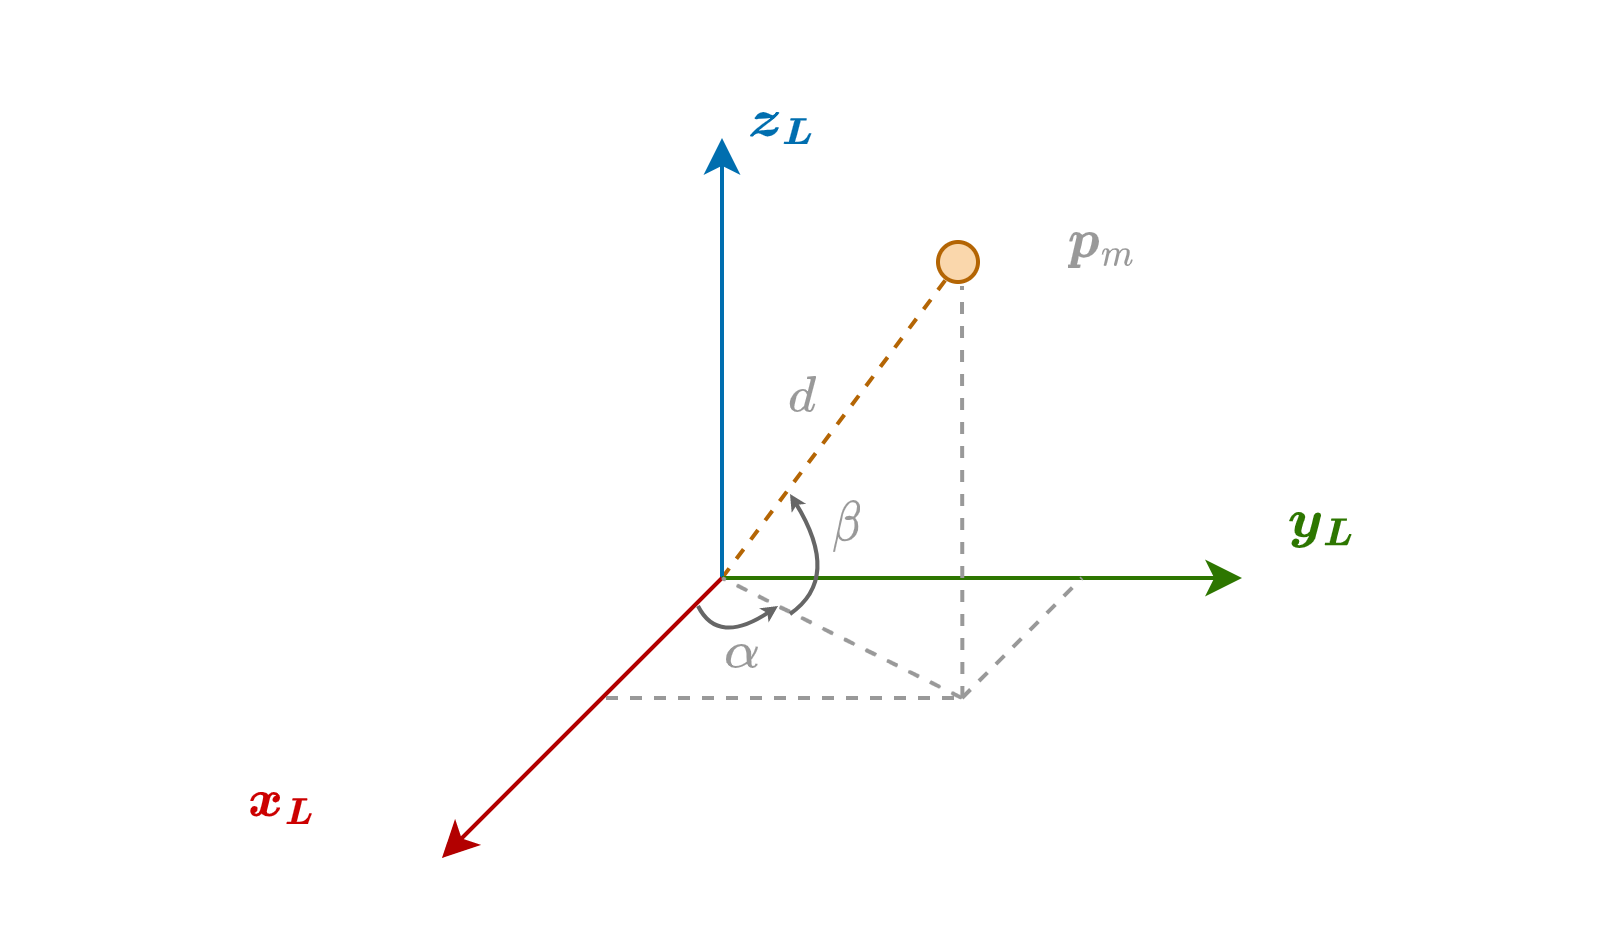
\includegraphics[width=0.48\linewidth]{img/lidar_model.png}
    %   \label{fig:lidar_model}
    % }
    % \subfigure[\normf{运动畸变}]{
    %   \centering
    %   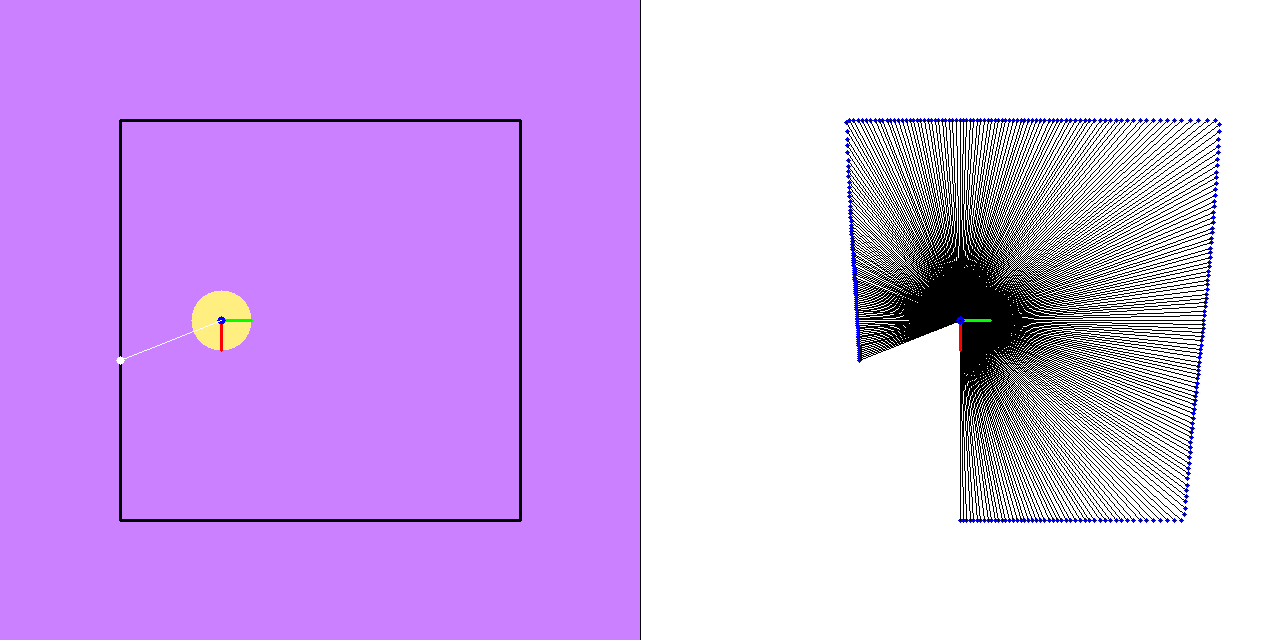
\includegraphics[width=0.48\linewidth]{img/lidar_motion_distort.png}
    %   \label{fig:lidar_motion_distort}
    % }
    \begin{subfigure}{0.48\textwidth}
      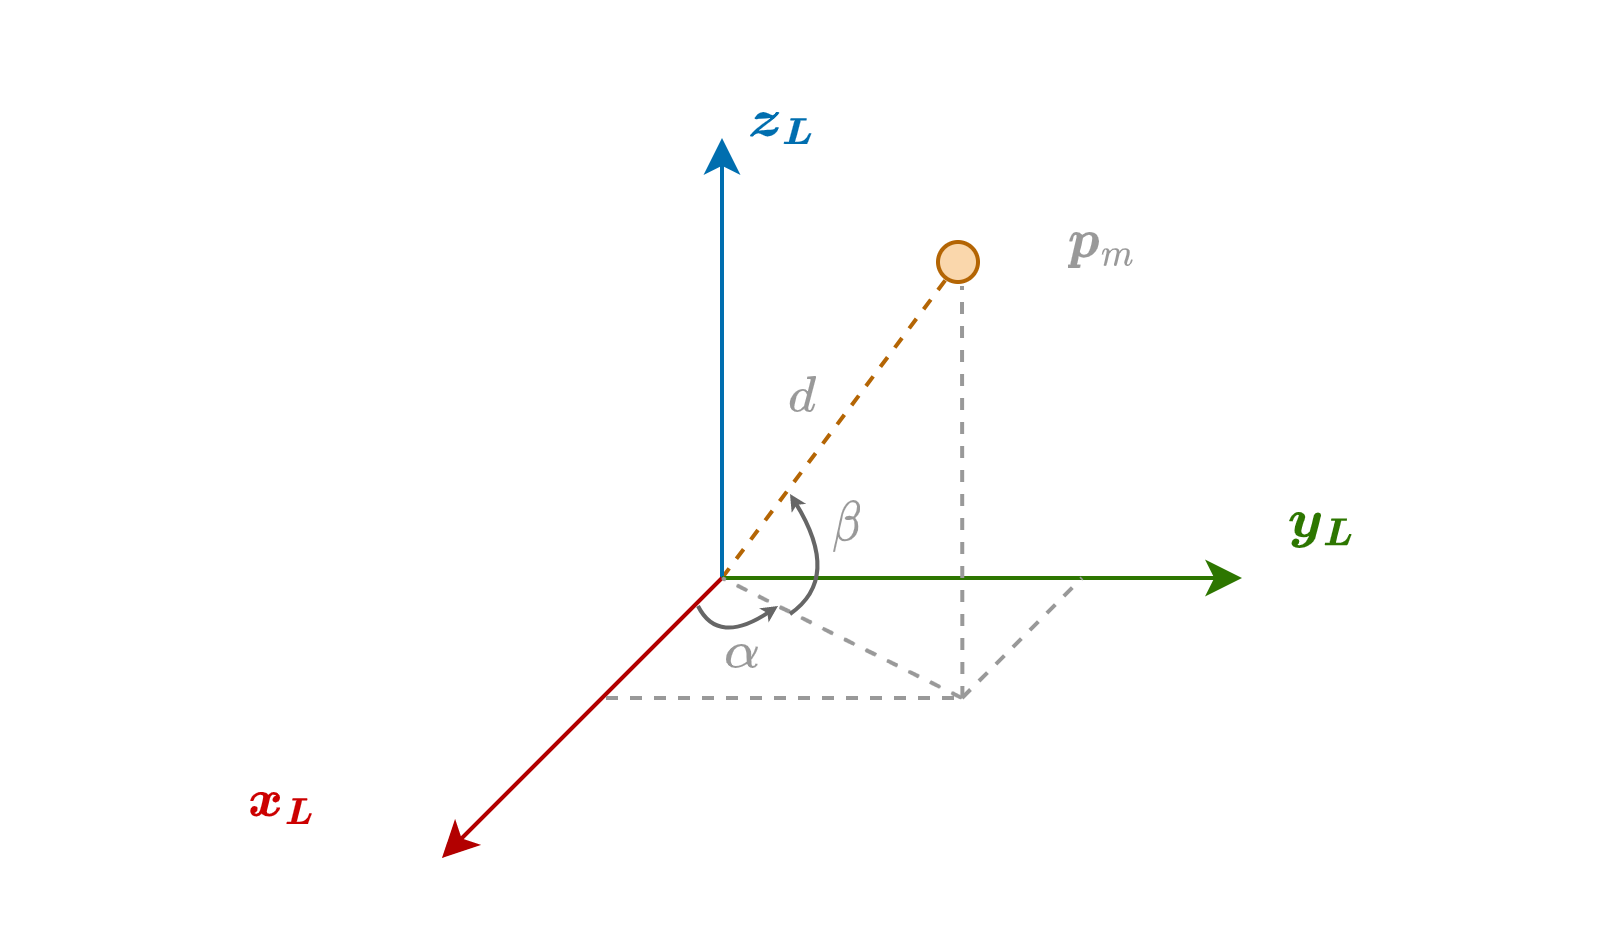
\includegraphics[width=\linewidth]{img/lidar_model.png}
      \caption{量测模型}
      \label{fig:lidar_model}
    \end{subfigure}
    \begin{subfigure}{0.48\textwidth}
      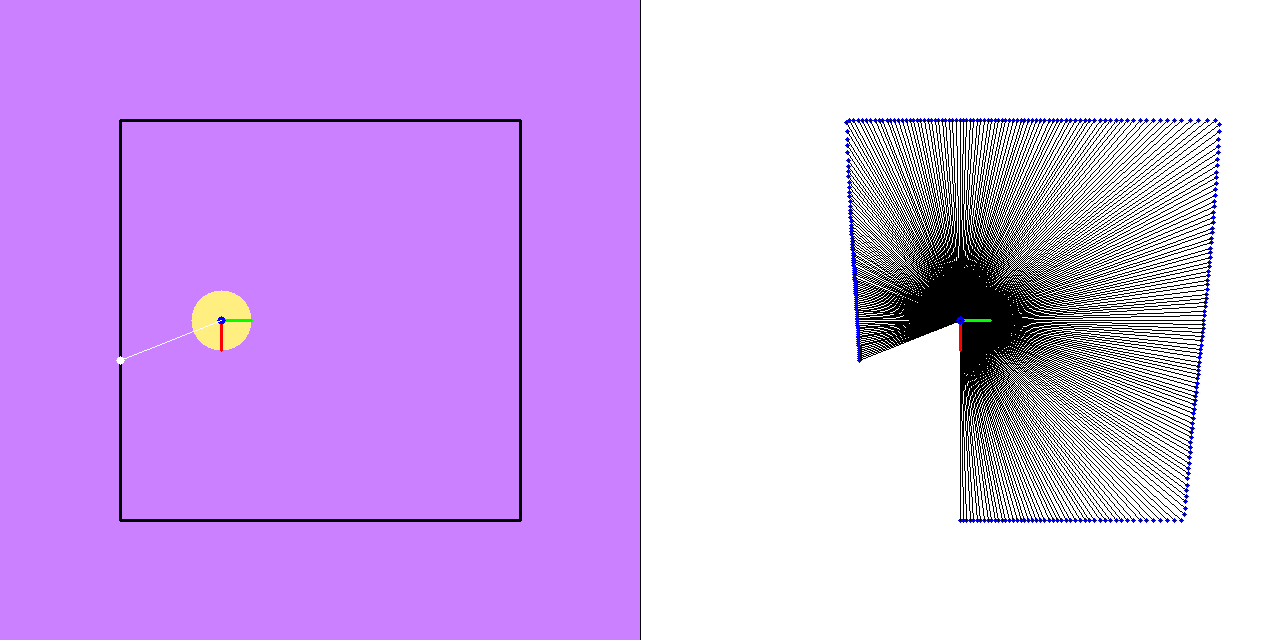
\includegraphics[width=\linewidth]{img/lidar_motion_distort.png}
      \caption{运动畸变}
      \label{fig:lidar_motion_distort}
    \end{subfigure}

    \caption{\normf{机械式激光雷达量测模型和运动畸变}}

    \label{fig:lidar}
  \end{figure}
}

机械式激光雷达存在待校准的内部参数,如每个激光发射器的高度角偏差、相对于理想L系的偏移量、测距偏差等,这些参数可以最终包含到一个相似变换(Similarity Transformation)里:
\begin{equation}
  \begin{pmatrix}
    {^{L}\boldsymbol{p}} \\1
  \end{pmatrix}={^{L}_{l_i}\boldsymbol{S}}\cdot
  \begin{pmatrix}
    {^{l_i}\widetilde{\boldsymbol{p}}} \\1
  \end{pmatrix}
  \quad\mathrm{s.t.}\quad
  {^{L}_{l_i}\boldsymbol{S}}=\begin{pmatrix}
    s_d\cdot{^{L}_{l_i}\boldsymbol{R}} & {^{L}\boldsymbol{t}_{l_i}} \\\boldsymbol{0}&1
  \end{pmatrix}\quad
  {^{l_i}\widetilde{\boldsymbol{p}}}=\begin{pmatrix}
    \widetilde{d}\times\cos\widetilde{\alpha}\times\cos\widetilde{\beta} \\
    \widetilde{d}\times\cos\widetilde{\alpha}\times\sin\widetilde{\beta} \\
    \widetilde{d}\times\sin\widetilde{\alpha}
  \end{pmatrix}
\end{equation}
其中:${^{l_i}\widetilde{\boldsymbol{p}}}$为根据目标点在第$i$个激光发射器坐标系下测得的距离$\widetilde{d}$、旋转角$\widetilde{\alpha}$和高度角$\widetilde{\beta}$计算得到的点坐标;${^{L}_{l_i}\boldsymbol{S}}$为第$i$个激光发射器坐标系$l_i$到理想雷达坐标系L的相似变换矩阵,相较于刚体变换多了一个关于测程$d$的尺度因子$s_d$。在实际应用中,由于这些偏差数值较小,影响有限且在可接受范围内,所以本文不考虑这些参数的标定,即认为机械式激光雷达为理想模型,其量测模型严格满足式\ref{equ:lidar_model}。

\subsection{\normf{Camera}}
相机可以将三维空间中的场景映射到二维像平面上,其和LiDAR一样,也是一种外部传感器。相机的成像模型较多,有针孔相机模型、等距相机模型、全向相机模型等,本文只讨论最简单的针孔相机模型。

针孔相机的成像模型所图\ref{fig:camera_model}所示。对于空间中的一物方点$\boldsymbol{p}_w$,其在像平面上的成像点为$\boldsymbol{p}_i$,则物方点$\boldsymbol{p}_w$、成像点$\boldsymbol{p}_i$和相机光心$\boldsymbol{O}$三点共线,即有:
\begin{equation}
  \label{equ:collinear}
  \frac{z_w}{f}=-\frac{y_w}{y_i}=-\frac{x_w}{x_i}\quad\to\quad
  \begin{cases}
    \begin{aligned}
      x_i & =-f\times\frac{x_w}{z_w} \\
      y_i & =-f\times\frac{y_w}{z_w}
    \end{aligned}
  \end{cases}
\end{equation}
其中$f$为相机的焦距,其值等于相机光心$\boldsymbol{O}$到像平面的垂直距离。对原始影像取倒像,可以将式\ref{equ:collinear}中的负号去除,该操作等价于将像平面挪到相机光心前面。像平面上点一般在像素坐标系下表达,坐标系原点$o$定义在图像的左上角,水平向右为$u$轴,垂直向下为$v$轴,构成平面$o$-$u$-$v$坐标系。

结合式\ref{equ:collinear},同时考虑像素大小和物理尺寸在横纵方向上的比例因子$s_x$、$s_y$(单位为:像素/$m$),可以得到:
\begin{equation}
  \label{equ:cam_pinhole}
  \begin{cases}
    \begin{aligned}
      u & =s_x\times f\times\frac{x_w}{z_w}+c_x \\
      v & =s_y\times f\times\frac{y_w}{z_w}+c_y
    \end{aligned}
  \end{cases}\to\quad
  \begin{cases}
    \begin{aligned}
      u & =f_x\times x_n+c_x \\
      v & =f_y\times y_n+c_y
    \end{aligned}
  \end{cases}\to\quad
  \begin{pmatrix}
    u \\v\\1
  \end{pmatrix}=\begin{pmatrix}
    f_x & 0   & c_x \\
    0   & f_y & c_y \\
    0   & 0   & 1
  \end{pmatrix}\begin{pmatrix}
    x_n \\y_n\\1
  \end{pmatrix}
\end{equation}
其中:$\boldsymbol{c}\left( c_x,c_y\right) $为相机光心在像平面上投影点(即像主点)的像素坐标;$\boldsymbol{p}_n\left(
  x_n,y_n\right) $为物方点$\boldsymbol{p}_w$在相机归一化平面\footnote{\normf{将相机坐标系下的点的Z坐标归1,即可将该点转换到相机归一化平面上。注意到,相机归一化平面上的点各维单位均为1。}}上的投影点;$\boldsymbol{p}\left(u,v \right) $为位于像平面上的成像点;$f_x$、$f_y$分别为横向和纵向上的缩放因子,简称为像素焦距,单位为像素。为方便后续表示,记$\boldsymbol{K}$为相机的内参矩阵,则将相机坐标系$C$下表达的物方点${^{C}\boldsymbol{p}_w}$投影到像平面上点$\boldsymbol{p}$的过程为:
\begin{equation}
  z_w\cdot\begin{pmatrix}
    \boldsymbol{p} \\1
  \end{pmatrix}=\boldsymbol{K}\cdot{^{C}\boldsymbol{p}_w}
  \quad\mathrm{s.t.}\quad
  \boldsymbol{K}=\begin{pmatrix}
    f_x & 0   & c_x \\
    0   & f_y & c_y \\
    0   & 0   & 1
  \end{pmatrix}
\end{equation}

相机在成像过程中,会受到透镜制造工艺和安装误差的影响,导致畸变效应的产生。对于针孔相机而言,一般将其建模为径向畸变和切向畸变\cite{高翔2017视觉},具体的公式如下:
\begin{equation}
  \label{equ:cam_pinhole_dist}
  \begin{cases}
    x_d=x_n(1+k_1r^2+k_2r^4+k_3r^6)+2p_1x_ny_n+p_2(r^2+2x_n^2) \\
    y_d=y_n(1+k_1r^2+k_2r^4+k_3r^6)+p_1(r^2+2y_n^2)+2p_2x_ny_n
  \end{cases}
\end{equation}
其中$r^2=x_n^2+y_n^2$为归一化平面上的点到该平面原点的距离平方,$\boldsymbol{p}_d\left( x_d,y_d	\right) $为加畸变后的点,其仍然位于归一化平面上。
%%%%%%%%%%%%%%%%%%%%%%%%%%%%%%%%%%%%%%%%%%%%%%%%%%%%%%%%%%%%%%%%%%%%%%%%%%%%%%%%%%%%%%%%%
\mlcomment{
  \begin{figure}[htbp]
    \centering

    \begin{subfigure}{0.48\textwidth}
      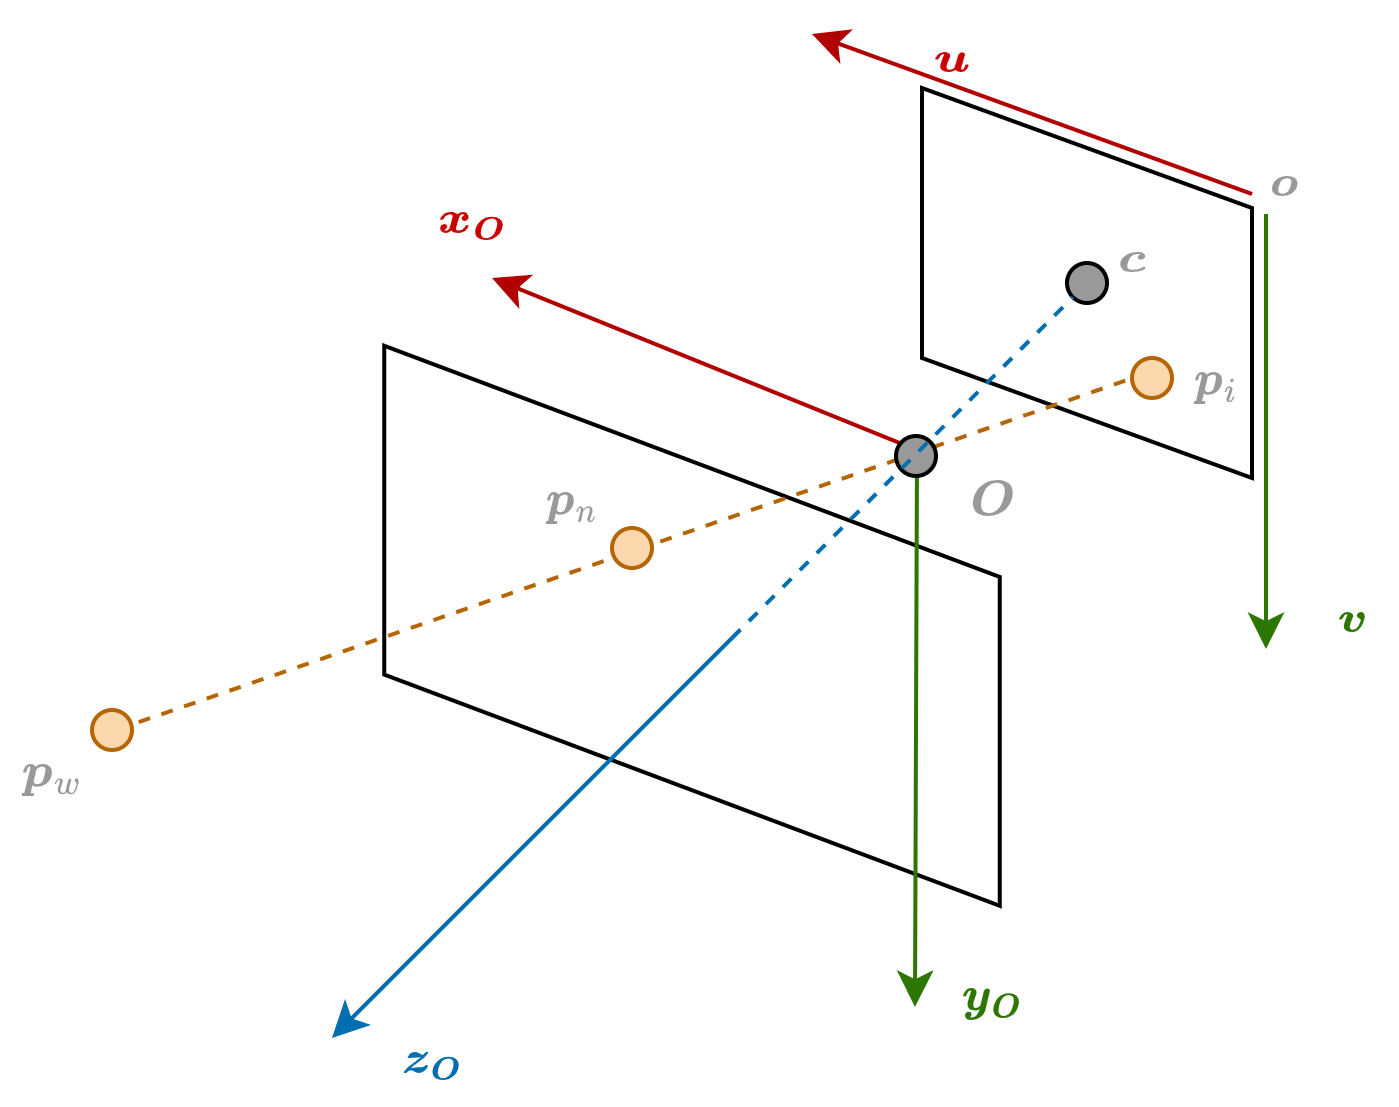
\includegraphics[width=\linewidth]{img/camera_model.png}
      \caption{量测模型}
      \label{fig:camera_model}
    \end{subfigure}
    \begin{subfigure}{0.48\textwidth}
      
\includegraphics[width=\linewidth]{img/rs_camera_distort.png}
      \caption{果冻效应}
      \label{fig:rs_camera_distort}
    \end{subfigure}

    % \subcaptionbox{\normf{量测模型}}{
    %   \centering
    %   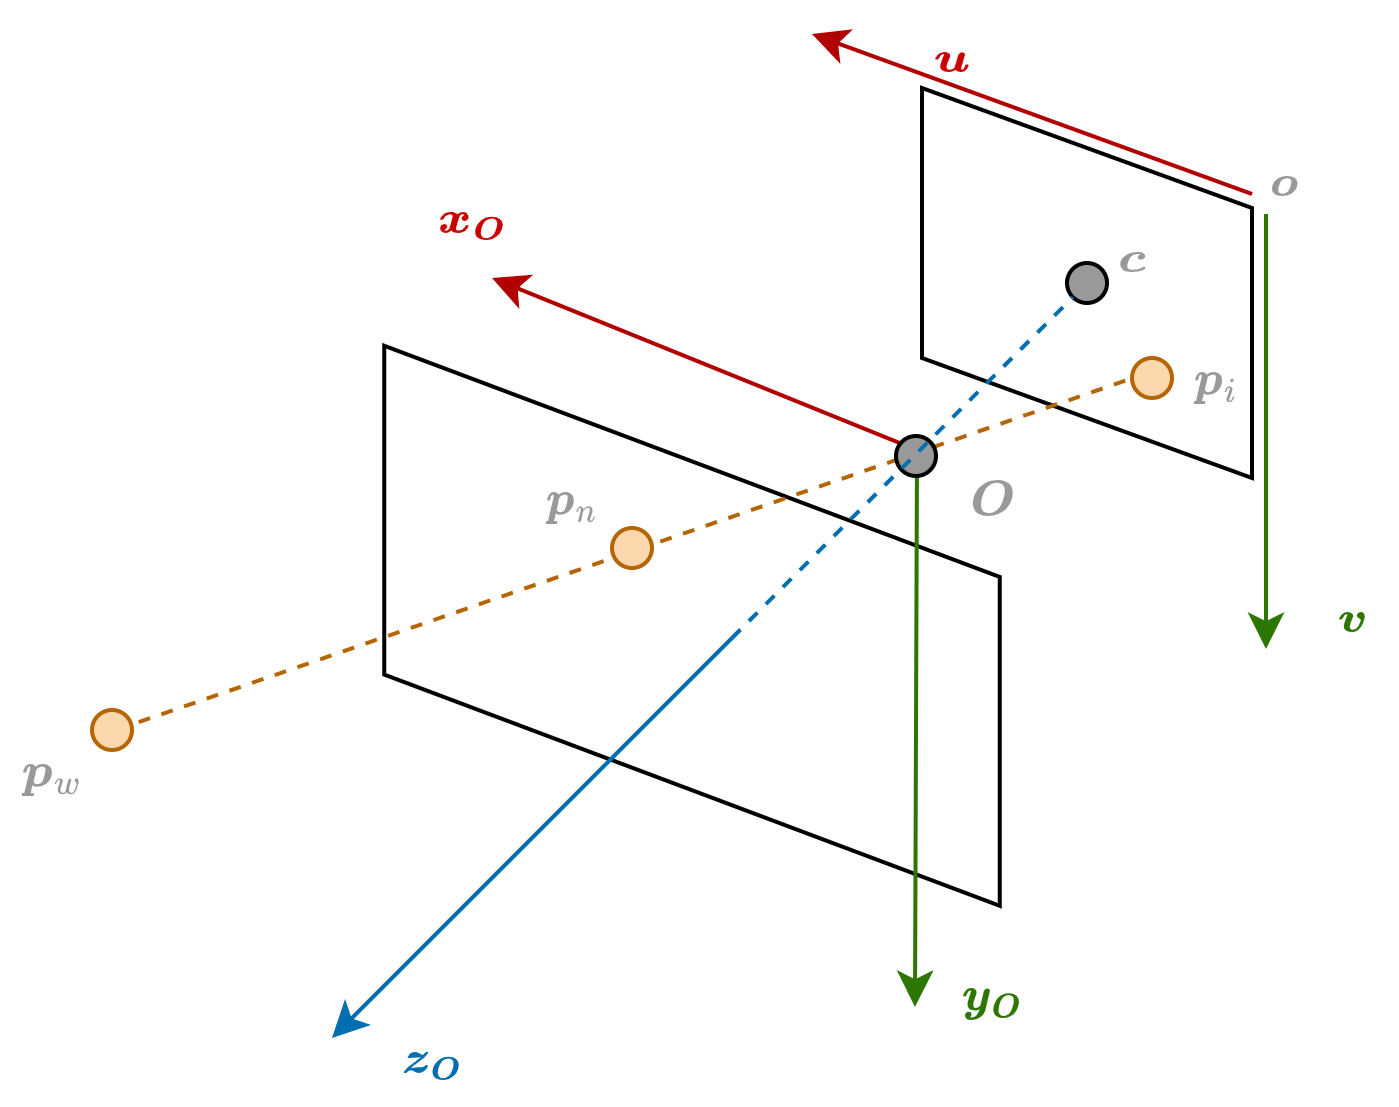
\includegraphics[width=0.48\linewidth]{img/camera_model.png}
    %   \label{fig:camera_model}
    % }
    % \subcaptionbox{\normf{果冻效应}}{
    %   \centering
    %   
\includegraphics[width=0.48\linewidth]{img/rs_camera_distort.png}
    %   \label{fig:rs_camera_distort}
    % }


    \caption{\normf{卷帘式针孔相机量测模型和果冻效应}}

    \label{fig:camera}
  \end{figure}
}

对于针孔相机而言,可以根据曝光方式的不同,将其分为全局曝光相机(Global Shutter)和卷帘快门相机(Rolling Shutter)。全局曝光相机在同一时刻获取整幅影像上的像素强度;而卷帘快门相机则是通过行扫描的方式,在同一时刻获取单行的像素强度,因此同一幅影像上的不同行是异步采集的。相较于全局曝光相机,卷帘快门相机具有价格便宜、体积小、功耗低的优点,适合在移动平台上应用,比如手机、机器人、无人机等,因此本文标定使用的相机为卷帘快门相机\footnote{\normf{虽然本文研究的是卷帘快门相机,但是可以通过固定优化参数的方式,轻易地适配全局曝光相机。}}。

与机械激光雷达类似,卷帘快门相机的图像帧内是异步测量的,当场景中存在高速运动物体时,获取的影像存在畸变,称为果冻效应,如图\ref{fig:rs_camera_distort}所示。果冻效应会严重影响相关几何算法的精度,因此需要估计卷帘快门相机的读出时间(Readout Time)\footnote{\normf{即读出一幅图像帧总共所用的时间。由于读出单行时间是一致的,所以可以通过图像高度和行扫描时延计算得到。}}或行扫描时延(Line Delay)来去除畸变效应。


\subsection{\normf{IMU}}
惯性测量单元(Inertial Measurement Unit,IMU)由加速度计和陀螺仪组成。加速度计可以感知载体相对于惯性参考系的线加速度(即比力),陀螺仪则可以感知载体相对于惯性参考系的角速度。与激光雷达和相机不同,IMU是一种内部传感器,且其数据量更小,采样频率更高。根据实现原理的不同,加速度计和陀螺仪分为多种类别,本文使用的是MEMS惯性测量单元,其具有功率低、价格便宜的优点。

在对IMU进行建模时,本文主要考虑IMU的零偏(Bias)、比例因子(Scale Factor)和交轴耦合误差(Axis Misalignment),并顾及IMU的安装误差(IMU Misalignment)和量测噪声,即有:
\begin{equation}
  \label{equ:imu_model}
  \begin{cases}
    \begin{aligned}
      {^{G}}\boldsymbol{\omega}_m & =\boldsymbol{M}_\omega\cdot{^{G}_{I}\boldsymbol{R}}\cdot{^{I}}\boldsymbol{\omega}+\boldsymbol{b}_\omega+\boldsymbol{n}_\omega \\
      {^{A}}\boldsymbol{a}_m      & =\boldsymbol{M}_a\cdot{^{I}}\boldsymbol{a}+\boldsymbol{b}_a+\boldsymbol{n}_a
    \end{aligned}
  \end{cases}
\end{equation}
其中:${^{G}}\boldsymbol{\omega}_m$、${^{A}}\boldsymbol{a}_m$为陀螺仪和加速度计的原始输出;${^{I}}\boldsymbol{\omega}$、${^{I}}\boldsymbol{a}$为角速度和线加速度的理论值;$\boldsymbol{M}_{\omega\mid a}$矩阵包含了比例因子和交轴耦合误差(以加速度计为例,如图\ref{fig:imu_axis_mis}所示):
\begin{equation}
  \boldsymbol{M}_\omega=\begin{pmatrix}
    S_{\omega 1} & M_{\omega 1} & M_{\omega 2} \\
    0            & S_{\omega 2} & M_{\omega 3} \\
    0            & 0            & S_{\omega 3}
  \end{pmatrix}\quad \boldsymbol{M}_a=\begin{pmatrix}
    S_{a 1} & M_{a 1} & M_{a 2} \\
    0       & S_{a 2} & M_{a 3} \\
    0       & 0       & S_{a 3}
  \end{pmatrix}
\end{equation}
${^{G}_{I}\boldsymbol{R}}$为IMU的安装误差旋转矩阵(如图\ref{fig:imu_mis}所示)。本文以加速度计坐标系作为IMU坐标系,因此在处理角速度时,需要通过旋转矩阵${^{G}_{I}\boldsymbol{R}}$进行角速度向量的变换;$\boldsymbol{b}_\omega$、$\boldsymbol{b}_a$为陀螺仪和加速度计的零偏,本文建模为高斯随机游走;$\boldsymbol{n}_\omega$、$\boldsymbol{n}_a$分别为陀螺仪和加速度计的加性量测噪声,本文建模为零均值高斯白噪声。
%%%%%%%%%%%%%%%%%%%%%%%%%%%%%%%%%%%%%%%%%%%%%%%%%%%%%%%%%%%%%%%%%%%%%%%%%%%%%%%%%%%%%%%%%
\mlcomment{
  \begin{figure}[htbp]
    \centering

    \begin{subfigure}{0.48\textwidth}
      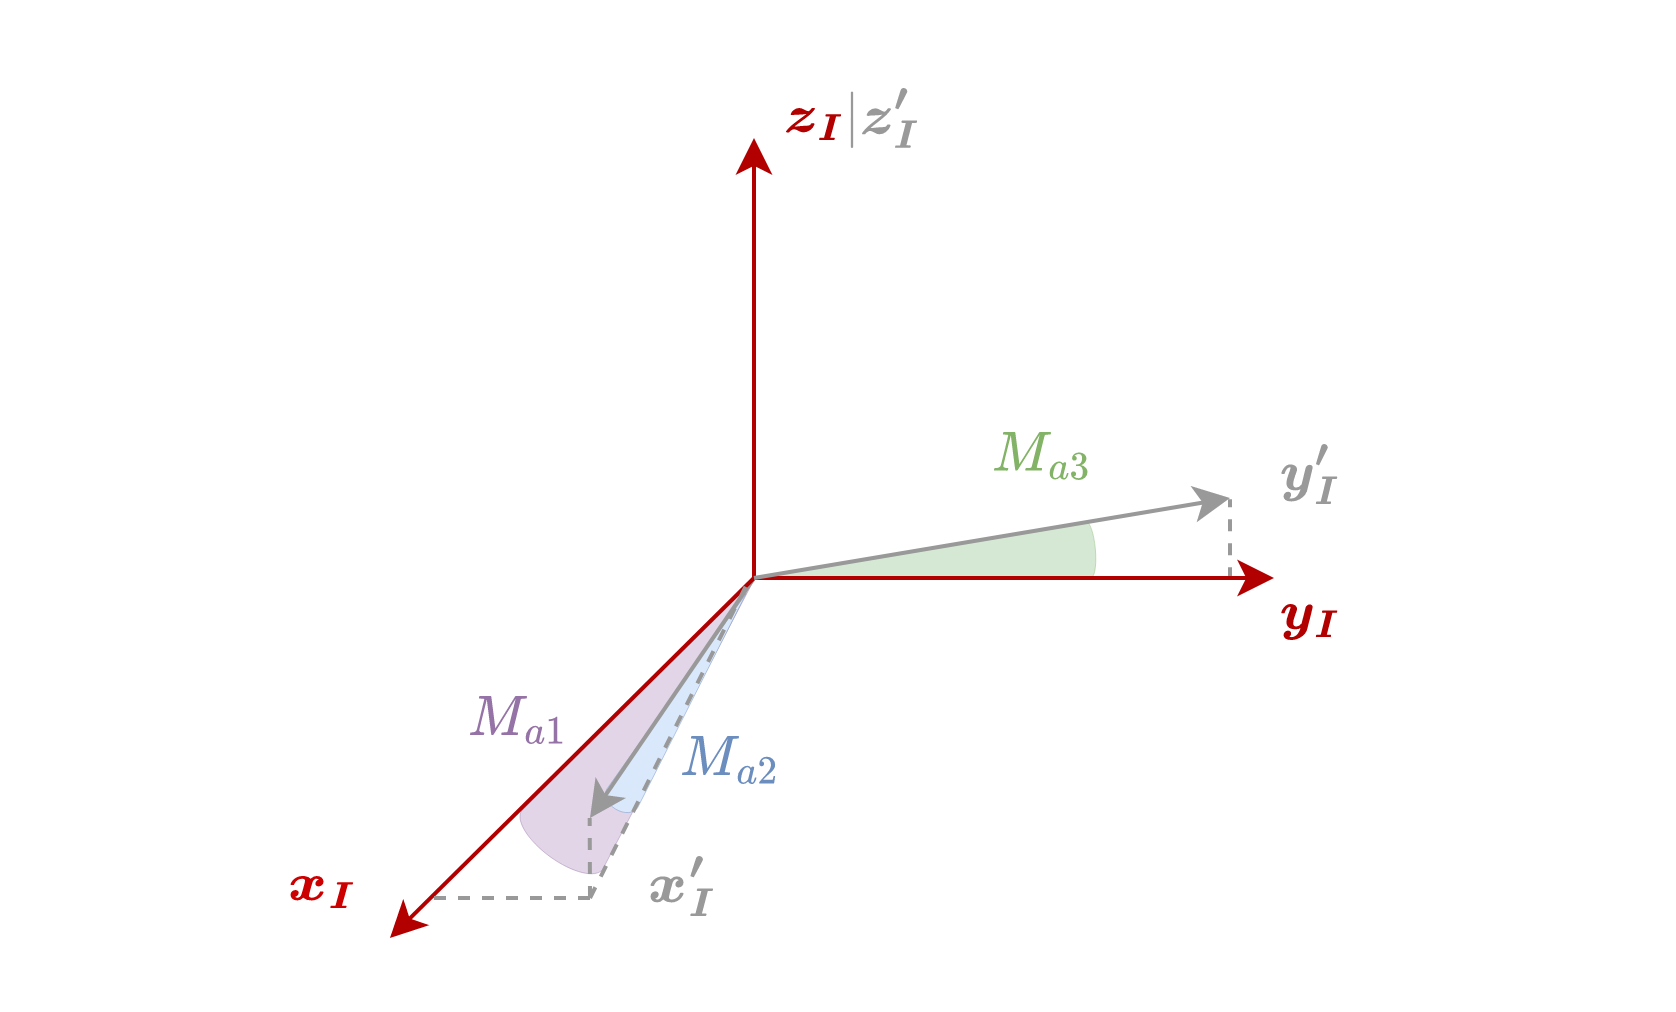
\includegraphics[width=\linewidth]{img/imu_axis_mis.png}
      \caption{交轴耦合误差}
      \label{fig:imu_axis_mis}
    \end{subfigure}
    \begin{subfigure}{0.48\textwidth}
      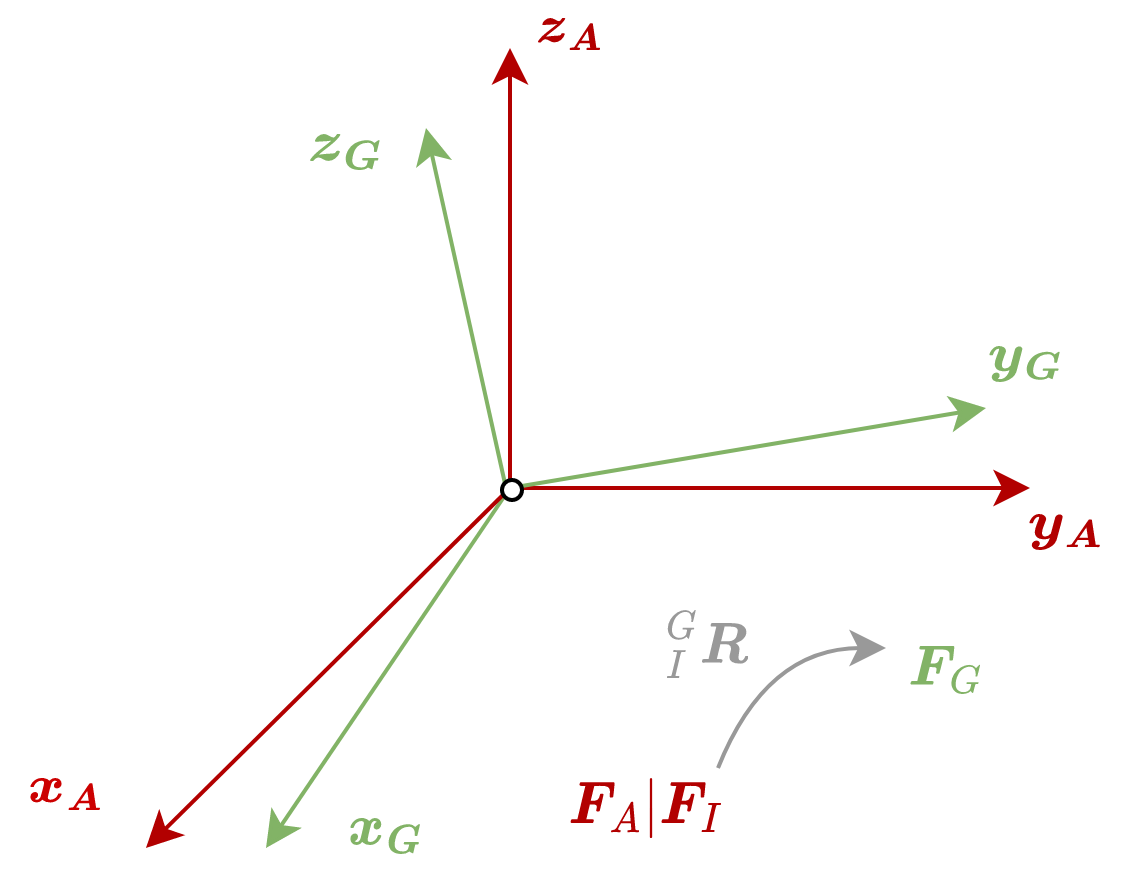
\includegraphics[width=\linewidth]{img/imu_mis.png}
      \caption{安装误差}
      \label{fig:imu_mis}
    \end{subfigure}
    % \subfigure[\normf{交轴耦合误差}]{
    %   \centering
    %   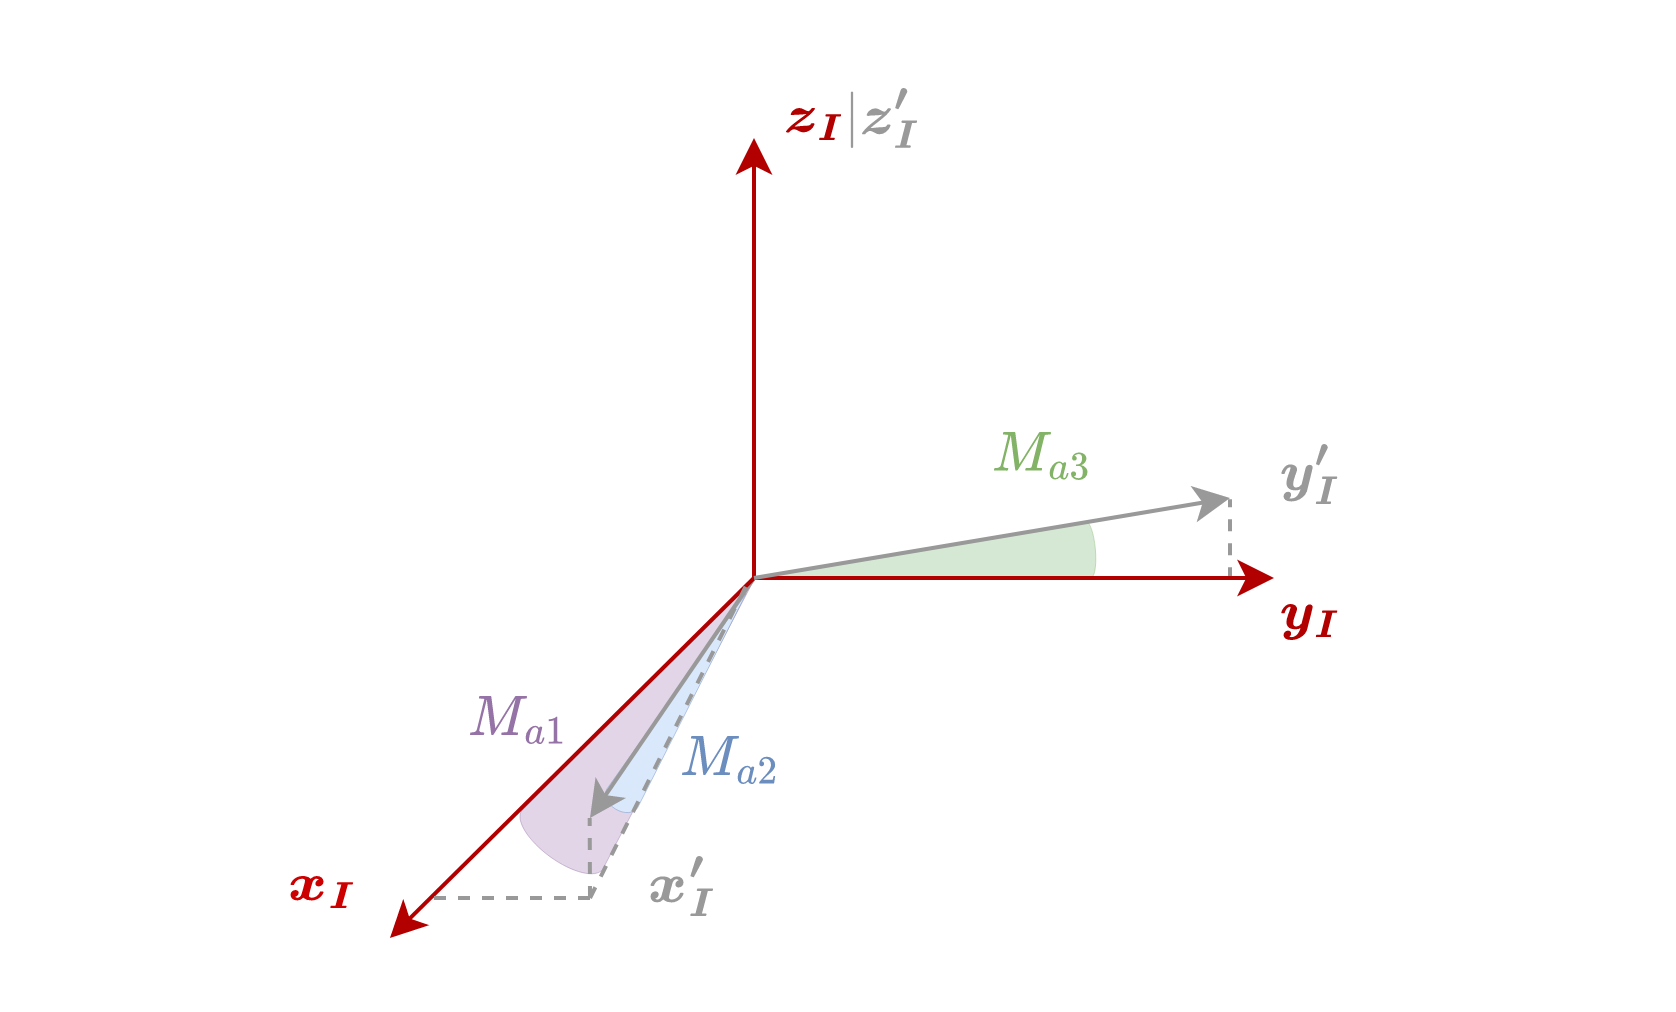
\includegraphics[width=0.48\linewidth]{img/imu_axis_mis.png}
    %   \label{fig:imu_axis_mis}
    % }
    % \subfigure[\normf{安装误差}]{
    %   \centering
    %   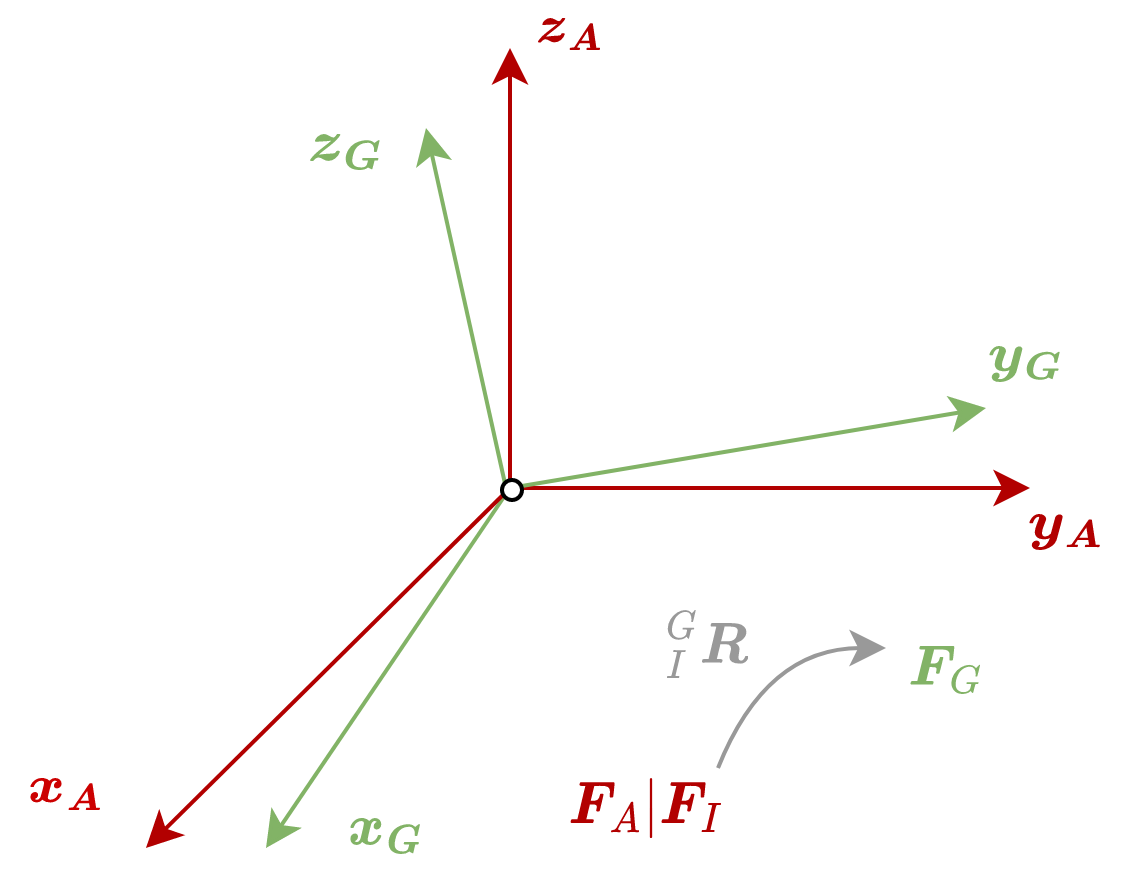
\includegraphics[width=0.48\linewidth]{img/imu_mis.png}
    %   \label{fig:imu_mis}
    % }

    \caption{\normf{IMU交轴耦合误差和安装误差}}

    \label{fig:imu}
  \end{figure}
}

\label{sensro_model_imu}

\subsection{\normf{待标参数}}
\label{suubsubsec:calib_param}
基于上文介绍的各传感器模型,下面给出本文标定框架中的待标参数:
\begin{enumerate}
  \item 外参

        外参描述不同传感器坐标系之间的变换关系,对于刚体变换而言,包含姿态量和平移量。本文待标外参有:
        \begin{itemize}
          \item $I$系与$L$系之间的外参:${^{I}_{L}}\boldsymbol{q}$、${^{I}}\boldsymbol{p}_{L}$;
          \item $I$系与$C$系之间的外参:${^{I}_{C}}\boldsymbol{q}$、${^{I}}\boldsymbol{p}_{C}$;
        \end{itemize}

  \item 内参

        内参描述传感器量测模型内部的映射关系,其具体形式取决于传感器的类型和量测模型建模方式。本文待标内参有:
        \begin{itemize}
          \item Camera内参:本文使用的相机模型为卷帘式针孔相机模型,在顾及相机的径向畸变和切向畸变下,内参有:像素焦距$f_x$、$f_y$,像主点像素坐标$c_x$、$c_y$,径向畸变参数$k_1$、$k_2$、$k_3$和切向畸变参数$p_1$、$p_2$。由于目前相机内参和畸变参数的标定算法已经成熟,故对于这些参数,本标定框架使用由粗到细(Coarse To Fine)的优化策略,基于给定初值进行精化;
          \item IMU内参:本文主要考虑IMU的安装误差旋转量${^{G}_{I}\boldsymbol{q}}$,加速度计和陀螺仪的比例因子和交轴耦合误差矩阵$\boldsymbol{M}_{a}$、$\boldsymbol{M}_{\omega}$,加速度计和陀螺仪的零偏$\boldsymbol{b}_a$、$\boldsymbol{b}_\omega$;
        \end{itemize}
        由于LiDAR内参偏差的影响在可接受范围内,故本文不予以考虑。
  \item 时参

        时参指与时间相关的参数。在进行粗略硬件同步的情况下,不同传感器时间系统之间会存在相对偏差,称为时延。时延的大小和传感器的设计、多传感器系统的架构、系统的运作环境\footnote{\normf{比如相机在不同亮度环境下采集图像,由于曝光时间的长短不同,会导致不同的时间偏差,这在本文的实测实验中也有体现(具体参考\ref{sec:exp_real_world}节)。}}等有关。另外对于卷帘快门相机,还存在读出时间。理论上读出时间属于和相机相关的参数,可以归为相机内参,但为了方便,本文将其划分为时参。基于此,本文待标时参有:
        \begin{itemize}
          \item IMU与LiDAR时参:$^{I}t_{L}$,IMU时间和LiDAR时间之间的转换关系为:$t_{I}=t_{L}+{^{I}t_{L}}$;
          \item IMU与Camera时参:$^{I}t_{C}$,IMU时间和Camera时间之间的转换关系为:$t_{I}=t_{C}+{^{I}t_{C}}$;
          \item
                卷帘快门相机读出时间:$t_{r}$,其定义方式与\cite{huai2022observability}一致,如图\ref{fig:gs_rs}所示。设图像帧的相机时间撮为图像首行的相机时间$t_C\left( 0\right)$,则对于第$v$行的像素,其相机时间为:
                \begin{equation}
                  \label{equ:readout_time}
                  t_C(v)=t_C\left( 0\right) +\frac{v}{h} \times t_r
                \end{equation}
                其中$h$为图像的高度。
        \end{itemize}

\end{enumerate}
\mlcomment{
  \begin{figure}[htbp]
    \centering
    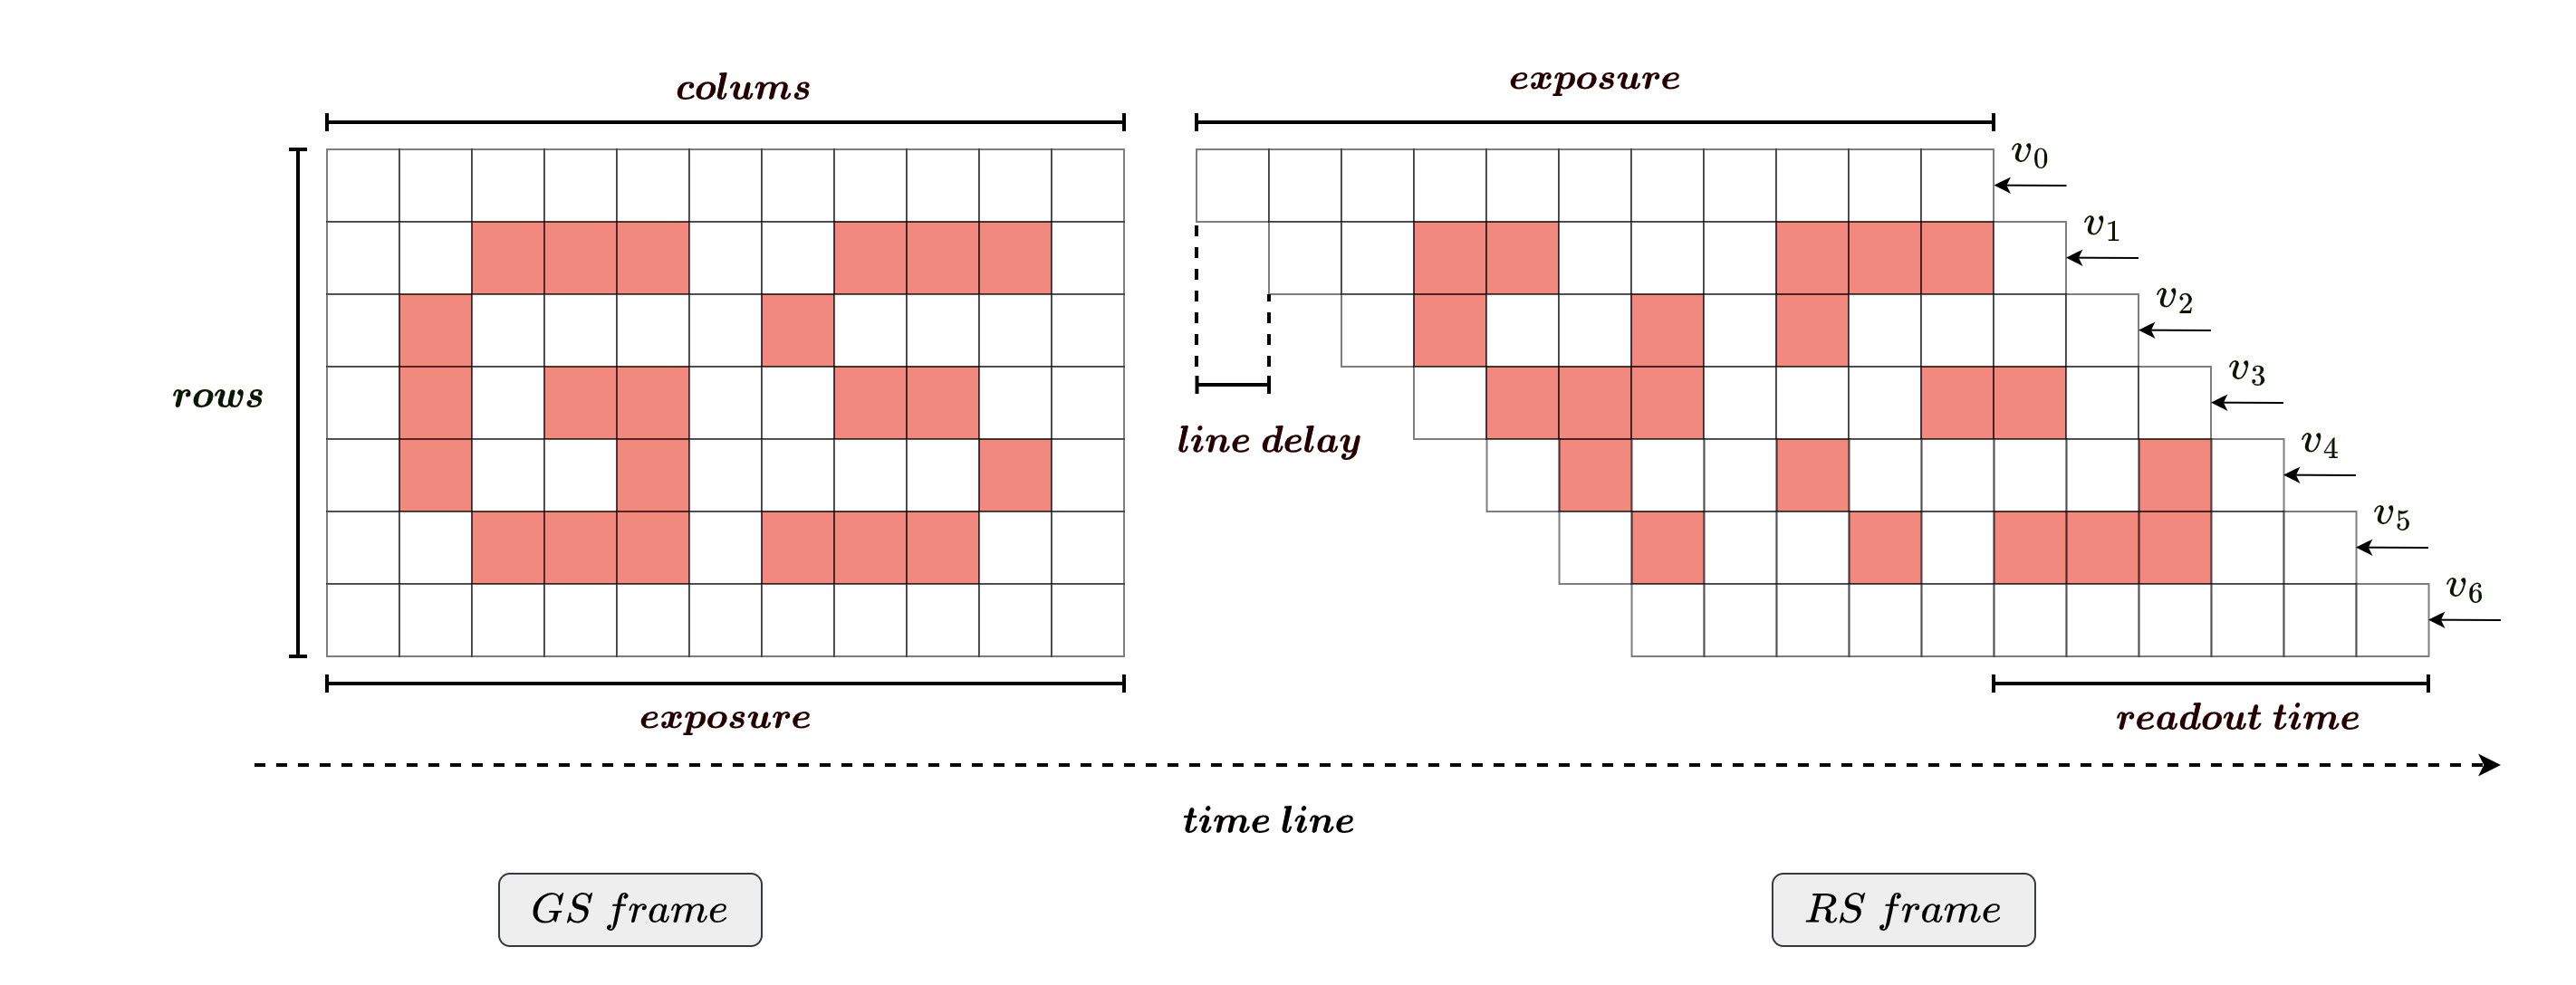
\includegraphics[width=0.95\linewidth]{img/gs_rs.png}

    \caption{\normf{GS相机全局曝光和RS相机行曝光}}

    \label{fig:gs_rs}
  \end{figure}
}

\section{\normf{连续时间理论}}
\subsection{\normf{离散时间和连续时间估计}}
本文所研究的标定算法是一种基于连续时间的无靶标标定方法,下面对离散时间理论和连续时间理论进行简要介绍。

真实世界中的传感器都是离散输出,如Camera和LiDAR输出帧率在10赫兹到30赫兹之间,IMU则可以达到上百赫兹。对于一个多传感器系统而言,在不考虑时延的情况下,直接处理不同传感器的同步离散输出来获取相关信息是一种简单有效的方法。但是当存在传感器异步测量时,需要进行时间同步,以消除异步测量带来的影响。一般而言,可以通过特制器件在硬件层面实现多传感器时间同步,但是这往往会增加系统的复杂度,成本也会更高。另一种时间同步方法是使用单一的中央处理单元(Central Processing Unit,CPU)记录不同传感器采集的数据帧的时间撮,在去除通信延迟后基于估计得到的常值时延进行时间同步。

对于后一种时间同步方法,目前存在两类方法:离散时间估计和连续时间估计。离散时间估计需要定制算法,以在估计过程中包含来自不同传感器的异步测量,且通常伴有相应的简化假设;而连续时间估计会先基于传感器的离散输出构建一个时间连续的函数,如B样条函数。当存在异步测量时,只需要对该函数进行采样,即可获取同步测量。

以机械激光雷达的运动畸变为例,由于同一点云帧中的不同点是异步测量,当LiDAR动态采集点云数据时,会导致畸变效应,因此需要进行时间同步。此时,离散时间估计方法一般会将运动简化为匀速运动或匀加速运动,而后基于已有的离散轨迹进行内插,如图\ref{fig:disc}所示。显然,当运动激烈时,这会引入较大的偏差。而连续时间估计方法会首先基于离散轨迹获取一个时间连续轨迹,如图\ref{fig:cont}所示,而后基于点云帧内各点的时间撮进行采样,并基于此消除运动畸变。
%%%%%%%%%%%%%%%%%%%%%%%%%%%%%%%%%%%%%%%%%%%%%%%%%%%%%%%%%%%%%%%%%%%%%%%%%%%%%%%%%%%%%%%%%
\mlcomment{
  \begin{figure}[htbp]
    \centering

    \begin{subfigure}{0.48\textwidth}
      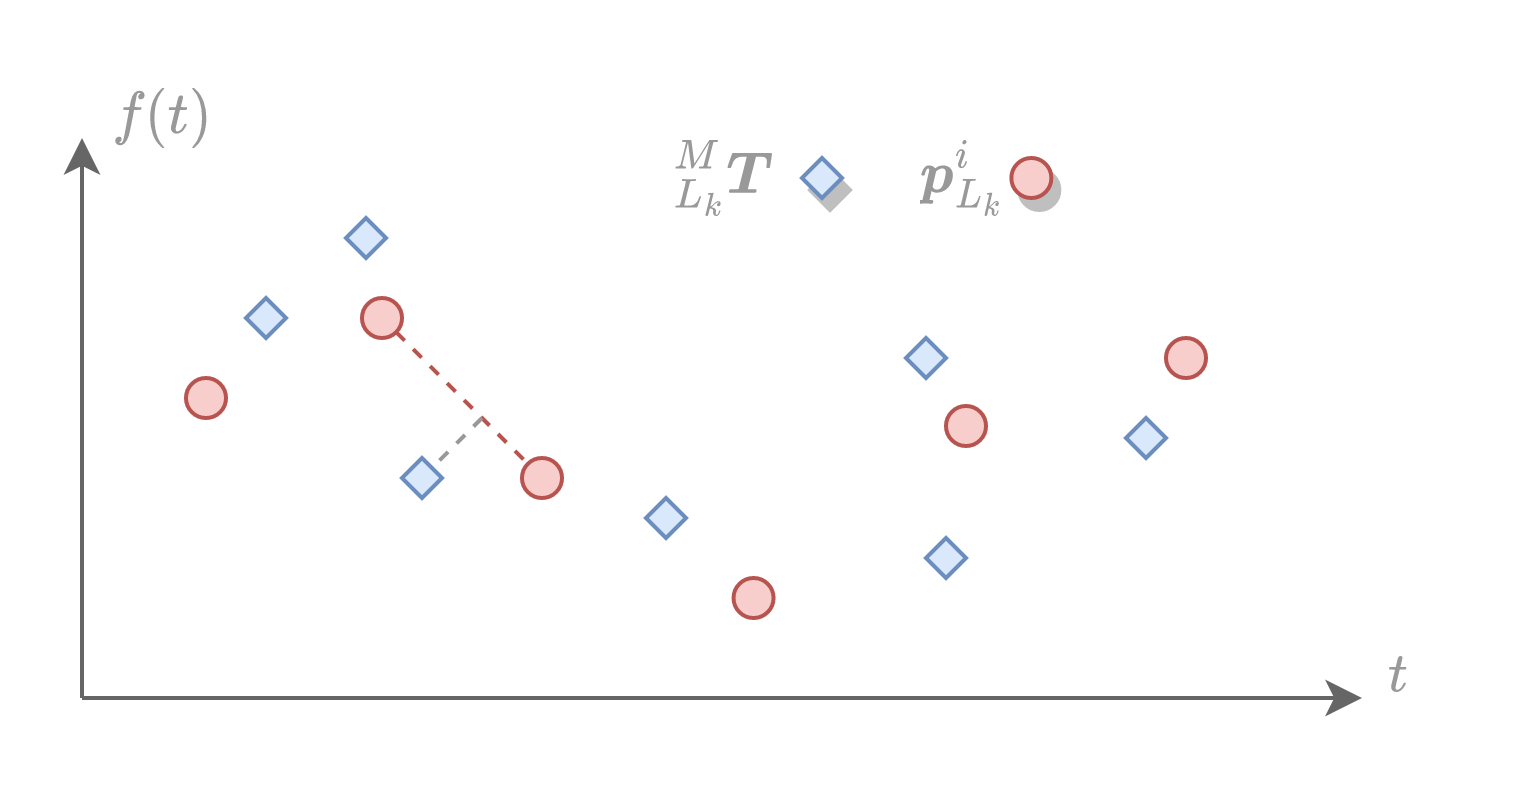
\includegraphics[width=\linewidth]{img/disc.png}
      \caption{离散时间估计}
      \label{fig:disc}
    \end{subfigure}
    \begin{subfigure}{0.48\textwidth}
      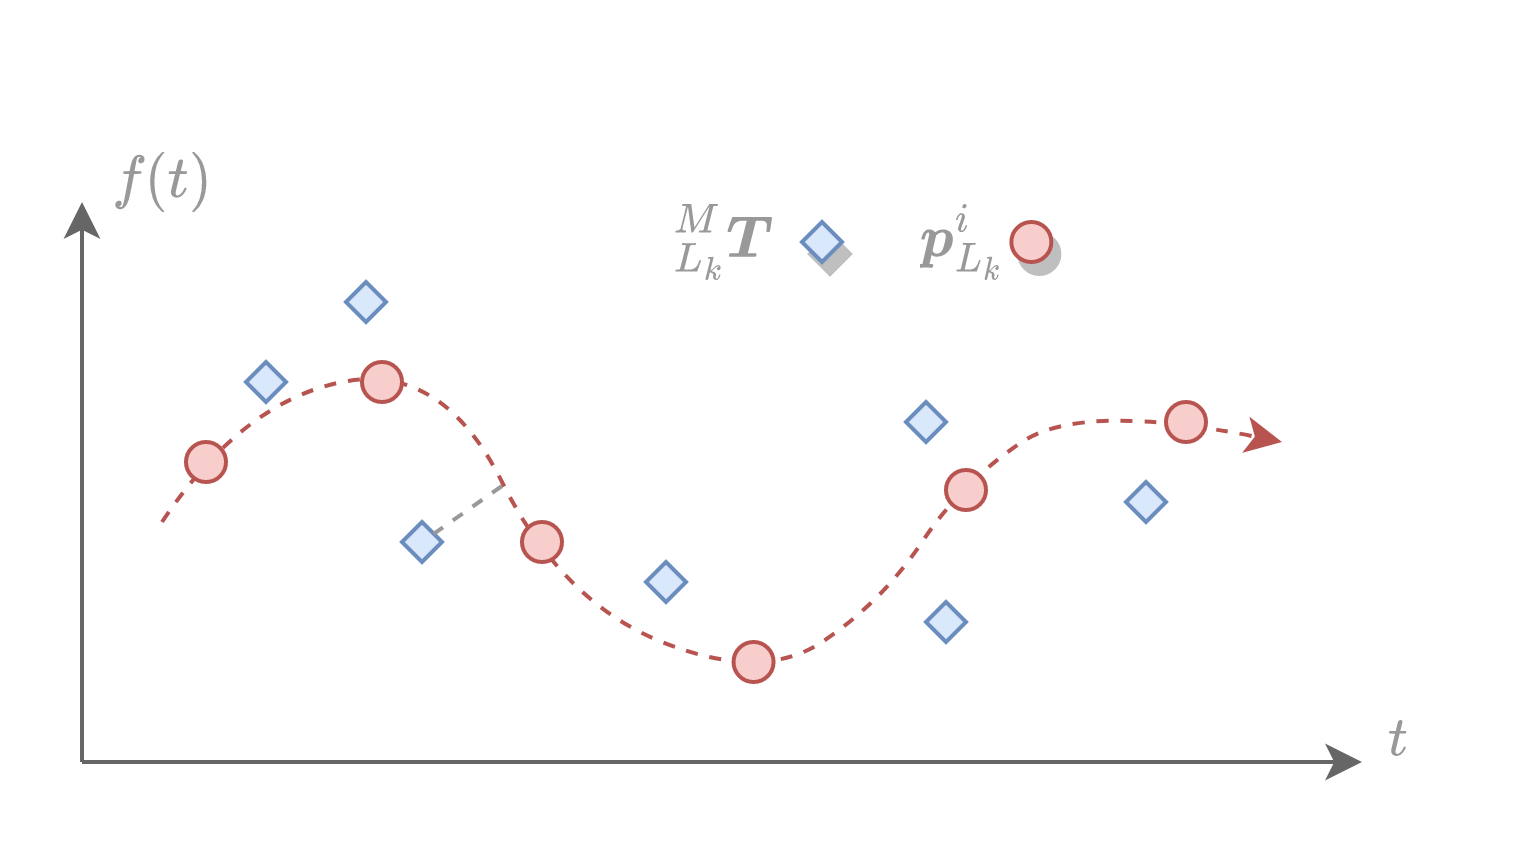
\includegraphics[width=\linewidth]{img/cont.png}
      \caption{连续时间估计}
      \label{fig:cont}
    \end{subfigure}
    % \subfigure[\normf{离散时间估计}]{
    %   \centering
    %   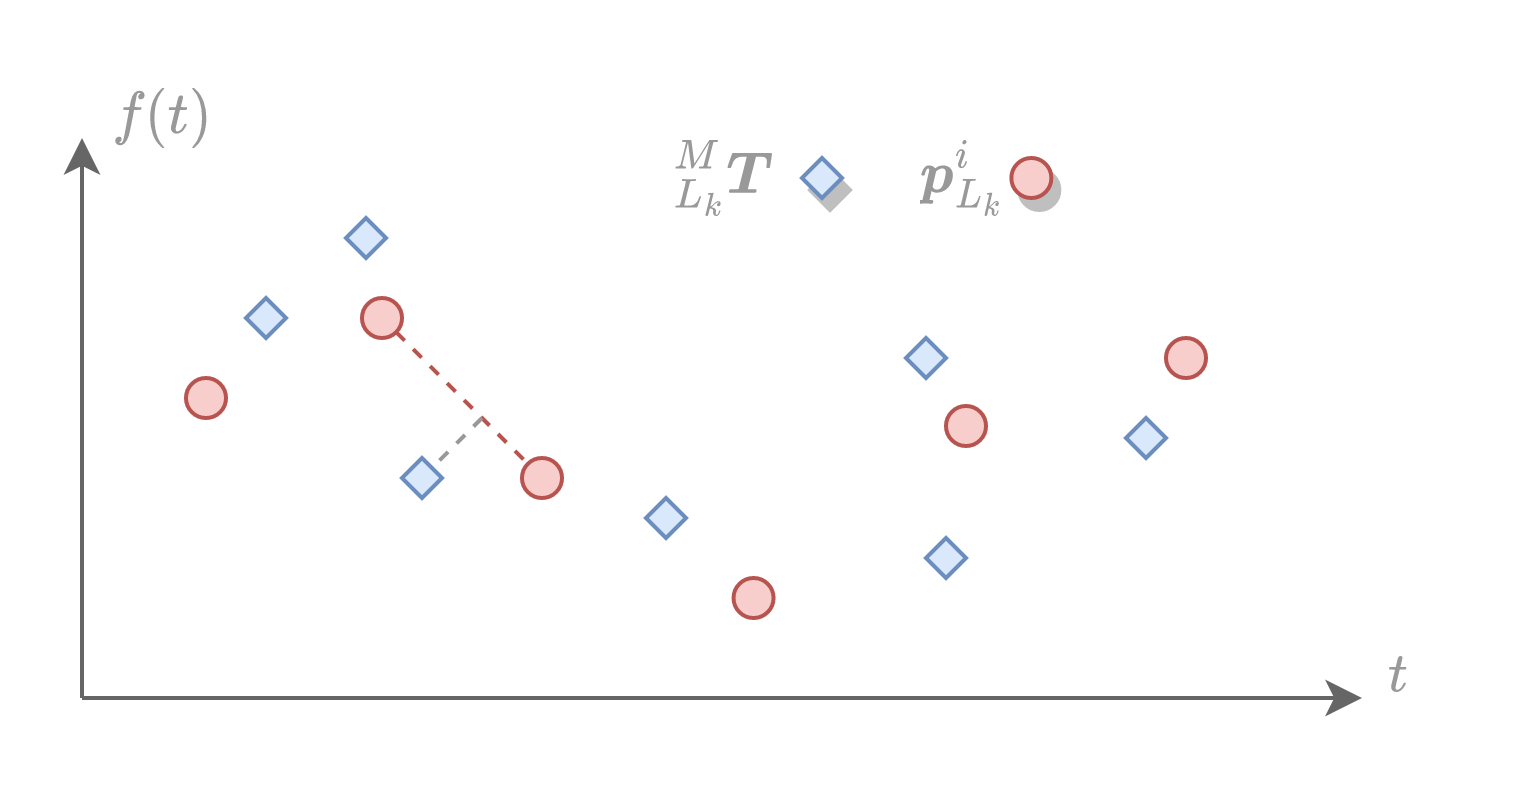
\includegraphics[width=0.48\linewidth]{img/disc.png}
    %   \label{fig:disc}
    % }
    % \subfigure[\normf{连续时间估计}]{
    %   \centering
    %   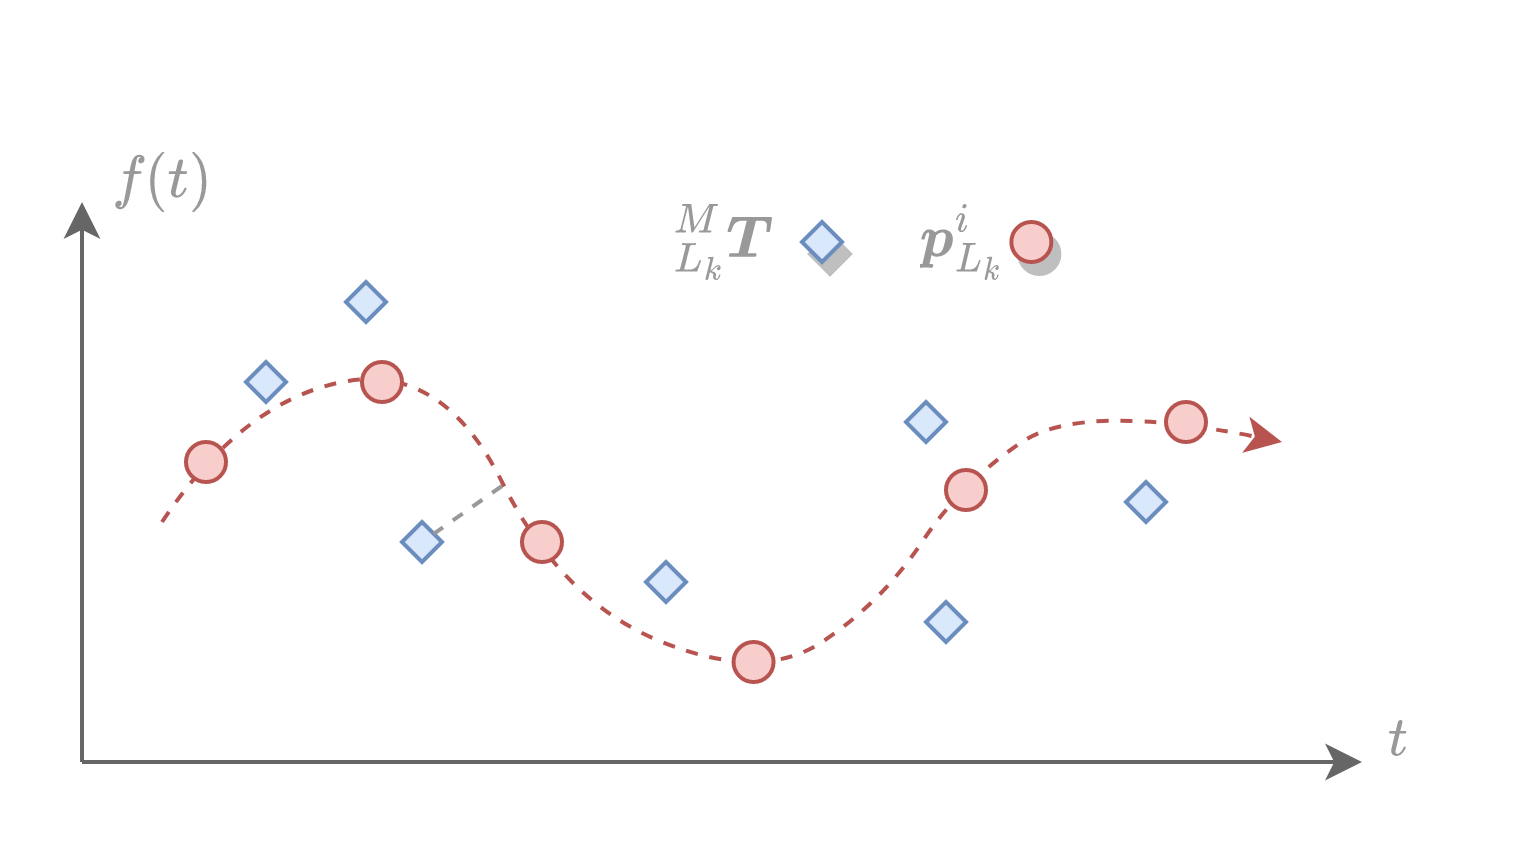
\includegraphics[width=0.48\linewidth]{img/cont.png}
    %   \label{fig:cont}
    % }

    \caption{\normf{基于离散时间估计和连续时间估计消除LiDAR帧运动畸变}}

    \label{fig:disc_cont}
  \end{figure}
}

事实上,已有研究表明:当不存在传感器异步测量时,离散时间估计和连续时间估计结果是一致的;当存在传感器异步测量时,连续时间估计要优于离散时间估计\cite{cioffi2022continuous}。由于本文标定算法涉及时参的标定,因此采用连续时间估计。
\subsection{\normf{B样条位姿曲线}}
\label{subsubsec:pose_bspline}
上文提到,在使用连续时间估计时需要基于时间离散数据构建时间连续的函数,本文使用B样条曲线进行时间连续建模,下面对其进行介绍。

B样条曲线诞生于计算机图形学领域,目的是为了在不损失精度的条件下,用离散的控制点和相关控制参数(即阶次)表示一条连续的曲线。B样条曲线是贝塞尔曲线的一种扩展。贝塞尔曲线通过离散的控制点和参数来控制曲线,但局部控制点的变动会影响整条曲线的走向,即贝塞尔曲线局部是不可控的。而B样条曲线是局部可控的,局部控制点的变动只会影响局部曲线,不会对其他区域的曲线造成影响,具有较强的操控性,因此应用较为广泛。对于一条具有$n+1$个控制点的$d$次B样条曲线\footnote{\normf{B样条曲线的阶数(order)比次数(degree)多1,即$d$次B样条曲线的阶为$d+1$。}},其可表示为:
\begin{equation}
  \label{equ:b_spline_origin}
  \boldsymbol{B}_{n,d}(t)=\sum_{i=0}^{n}\boldsymbol{p}_i\cdot b_{i,d}(t)
\end{equation}
其中$b_{i,d}(t)$可以通过Cox-de Boor递归公式\cite{de1978practical}得到:
\begin{equation}
  \begin{aligned}
    b_{i,0}(t) & =\begin{cases}
                    1\quad t_i\le t\le t_{i+1} \\
                    0\quad\dots
                  \end{cases}                                                                \\
    b_{i,d}(t) & =\frac{t-t_i}{t_{i+d}-t_i}b_{i,d-1}(t)+\frac{t_{i+d+1}-t}{t_{i+d+1}-t_{i+1}}b_{i+1,d-1}(t)
  \end{aligned}
\end{equation}
当节点等距时,称B样条均匀。均匀B样条完全由阶次决定,且$t\in[t_i,t_{i+1}]$节点处的值只由$d+1$个控制点$\boldsymbol{p}_i,\boldsymbol{p}_{i+1},\cdots,\boldsymbol{p}_{i+d}$约束。阶次决定了B样条曲线的表达能力,阶次越高,表达能力越强。图\ref{fig:bspline}展示了控制点相同但阶次不同的均匀B样条曲线。
%%%%%%%%%%%%%%%%%%%%%%%%%%%%%%%%%%%%%%%%%%%%%%%%%%%%%%%%%%%%%%%%%%%%%%%%%%%%%%%%%%%%%%%%
\mlcomment{
  \begin{figure}[htbp]
    \centering
    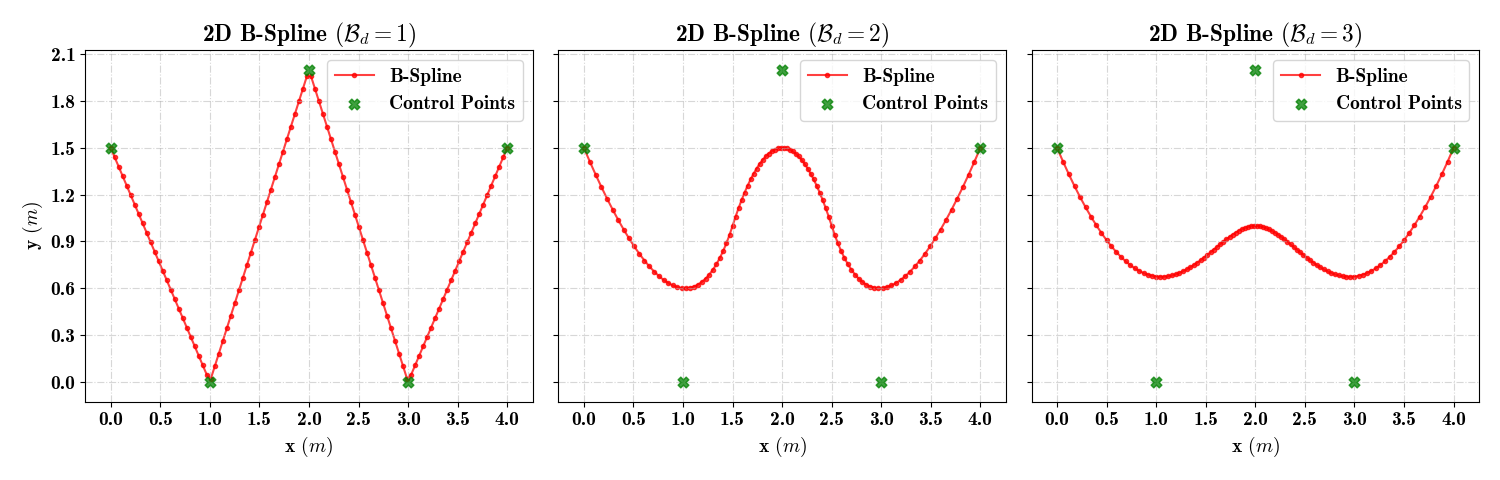
\includegraphics[width=0.95\linewidth]{img/bspline_2d.png}

    \caption{\normf{不同阶次的均匀B样条曲线比较}}

    \label{fig:bspline}
  \end{figure}
}

对于均匀B样条曲线而言,式\ref{equ:b_spline_origin}可以等价表示为更简洁的矩阵形式\cite{qin1998general}:
\begin{equation}
  \label{equ:matrix_bspline1}
  \boldsymbol{p}(t)=\sum_{j=0}^{d}\boldsymbol{u}^T\boldsymbol{M}^{(d+1)}_{(j)}\boldsymbol{p}_{i+j}
\end{equation}
其中:$\boldsymbol{u}^T=\begin{pmatrix}
    1 & u & \cdots & u^d
  \end{pmatrix}$,且$u=(t-t_i)/(t_{i+1}-t_i)$;$\boldsymbol{M}^{(d+1)}$是维度为$d+1$的方阵,$\boldsymbol{M}^{(d+1)}_{(j)}$表示其第$j$列。当$d$确定后,矩阵$\boldsymbol{M}^{(d+1)}$也就被唯一确定了。如在本文中,使用的是阶为4(即$d=3$)的B样条曲线表示轨迹,则:
\begin{equation}
  \boldsymbol{M}^{(3+1)}=\frac{1}{6}\begin{pmatrix}
    1  & 4  & 1  & 0 \\
    -3 & 0  & 3  & 0 \\
    3  & -6 & 3  & 0 \\
    -1 & 3  & -3 & 1
  \end{pmatrix}\quad
  \boldsymbol{u}=\begin{pmatrix}
    1\\{u}\\{u}^2\\{u}^3
  \end{pmatrix}
\end{equation}
进一步化简式\ref{equ:matrix_bspline1},可以得到:
\begin{equation}
  \label{equ:matrix_bspline2}
  \boldsymbol{p}(t)=\boldsymbol{p}_i+\sum_{j=1}^{d}\boldsymbol{u}^T\tilde{\boldsymbol{M}}^{(d+1)}_{(j)}(\boldsymbol{p}_{i+j}-\boldsymbol{p}_{i+j+1})
\end{equation}
当$d=3$时,上式中矩阵$\tilde{\boldsymbol{M}}^{(3+1)}$为:
\begin{equation}
  \tilde{\boldsymbol{M}}^{(3+1)}=\frac{1}{6}\begin{pmatrix}
    6 & 5  & 1  & 0 \\
    0 & 3  & 3  & 0 \\
    0 & -3 & 3  & 0 \\
    0 & 1  & -2 & 1
  \end{pmatrix}
\end{equation}

在使用均匀B样条曲线表示位姿轨迹时,可以采用姿态量和平移量分开的形式(即$\mathrm{SO}(3)+\mathbb{R}^3$),也可以采用二者耦合的形式(即SE(3))。后一种的精度更高,但其姿态量和平移量高度耦合,不利于控制平移曲线。而使用前一种解耦的方式分开表达位姿轨迹,更利于参数估计\cite{haarbach2018survey}。对于平移量,用式\ref{equ:matrix_bspline1}或式\ref{equ:matrix_bspline2}即可直接表示,但是对于姿态量而言,由于其在流行上其对数乘(本质上为加法)不封闭,需要作进一步处理\cite{高翔2017视觉}。具体而言,若用单位四元数表示姿态,则首先通过对数映射将旋转量从流行空间变换到代数空间,在数乘运算结束后通过指数映射回到流行空间,具体的推导可参考\cite{kim1995general}。这里直接给出结果:
\begin{equation}
  \boldsymbol{q}(t)=\boldsymbol{q}_i\circ \prod_{j=1}^{d}\exp\left( \boldsymbol{u}^T\tilde{\boldsymbol{M}}^{(d+1)}_{(j)}\log\left( \boldsymbol{q}_{i+j+1}^{-1}\circ \boldsymbol{q}_{i+j}\right) \right)
\end{equation}
其中$\circ$表示四元数乘法运算。

当使用均匀B样条曲线建立了时间连续的轨迹后,除了可以查询任意有效时刻的位姿外,还可以通过时间微分得到更高阶的轨迹信息,如速度、加速度、角速率等参量。比如,当使用IMU的离散位姿轨迹构建B样条曲线时,有:
\begin{equation}
  \label{equ:imu_bspline}
  \begin{cases}
    \begin{aligned}
      {^{I}\boldsymbol{a}(t)}      & ={^{I_0}_{I}\boldsymbol{R}^T(t)}\cdot({^{I_0}\ddot{\boldsymbol{p}}_I(t)}-{^{I_0}\boldsymbol{g}}) \\
      {^{I}\boldsymbol{\omega}(t)} & ={^{I_0}_{I}\boldsymbol{R}^T(t)}\cdot{^{I_0}_{I}\dot{\boldsymbol{R}}(t)}
    \end{aligned}
  \end{cases}
\end{equation}
其中:${^{I_0}\boldsymbol{g}}\in\mathbb{R}^3$表示首个IMU坐标系下的重力向量,在本文中将其模长设为常数$\vert \vert{^{I_0}\boldsymbol{g}}\vert\vert\approx 9.81m/s^2$,其自由度为2;${^{I_0}\ddot{\boldsymbol{p}}_I(t)}$表示$t$时刻的$I_t$系相对于$I_0$系的线加速度在$I_0$系下的表达;${^{I_0}_{I}\dot{\boldsymbol{R}}(t)}$表示$t$时刻的$I_t$系相对于$I_0$系的角速度在$I_0$系下的表达。

\section{\normf{因子图优化理论}}
\label{subsec:factor_graph}

从实现的角度出发,经典的优化估计问题可以分为两种:滤波方法和图优化方法。滤波方法一般基于马尔可夫性假设,计算效率高,但在处理非线性问题时会引入非线性误差。经典的滤波方法有卡尔漫滤波(Kalman Filter,KF)及其变种方法、粒子滤波(Particle Filter,PF)等。滤波方法的非线性误差可以通过迭代的方式多次线性化观测方程予以消除\cite{barfoot2017state},如迭代扩展卡尔漫滤波(Iterated Extended Kalman Filter,IEKF)。而图优化方法则在优化过程中多次线性化目标函数,更适合处理非线性问题,但计算效率稍低。图优化方法可以根据每次优化的规模,分为全局优化和局部优化\footnote{\normf{全局优化将所有待优化的参数一次性加入到优化图中进行优化估计,而局部优化则在优化过程中选择性地优化部分参数,其余参数被固定,不进行优化。SLAM领域经典的滑窗优化即为一种局部优化。}},后者只能保证局部最优,但是计算效率高。由于多传感器标定是一个高度非线性的问题,因此本文使用图优化方法进行参数估计。下面对图优化理论进行简单介绍。

对一个优化估计问题,可以通过分解的方式对其进行建模,如使用贝叶斯网络(Bayesian
Networks)、马尔可夫随机域(Markov Random Fields)、因子图(Factor Graphs)等。与贝叶斯网络使用概率密度建模不同,因子图通过因式分解的方式建模优化问题,因此可以将任何因子函数纳入到优化图中\cite{dellaert2017factor},如下所示:
\begin{equation}
  \label{equ:factor_graphs}
  p(x_1,x_2,\cdots,x_n)\propto\prod f_1(x_i,x_j,\cdots)\times f_2(x_j,x_k,\cdots)\times\cdots\times f_m(x_k,x_l,\cdots)
\end{equation}
其中$f_m$为因子函数,简称为因子;$x_n$为待优化变量,称为节点。优化的目标是使得式\ref{equ:factor_graphs}中的概率密度$p$最大,一般通过最大后验估计(Maximum A Posteriori,MAP)实现。因子图可以非常方便的表示因子化的过程,如对于式\ref{equ:factor_graphs}而言,其可表示为图\ref{fig:factor_graphs}所示的因子图。
%%%%%%%%%%%%%%%%%%%%%%%%%%%%%%%%%%%%%%%%%%%%%%%%%%%%%%%%%%%%%%%%%%%%%%%%%%%%%%%%%%%%%%%%%
\mlcomment{
  \begin{figure}[htbp]
    \centering
    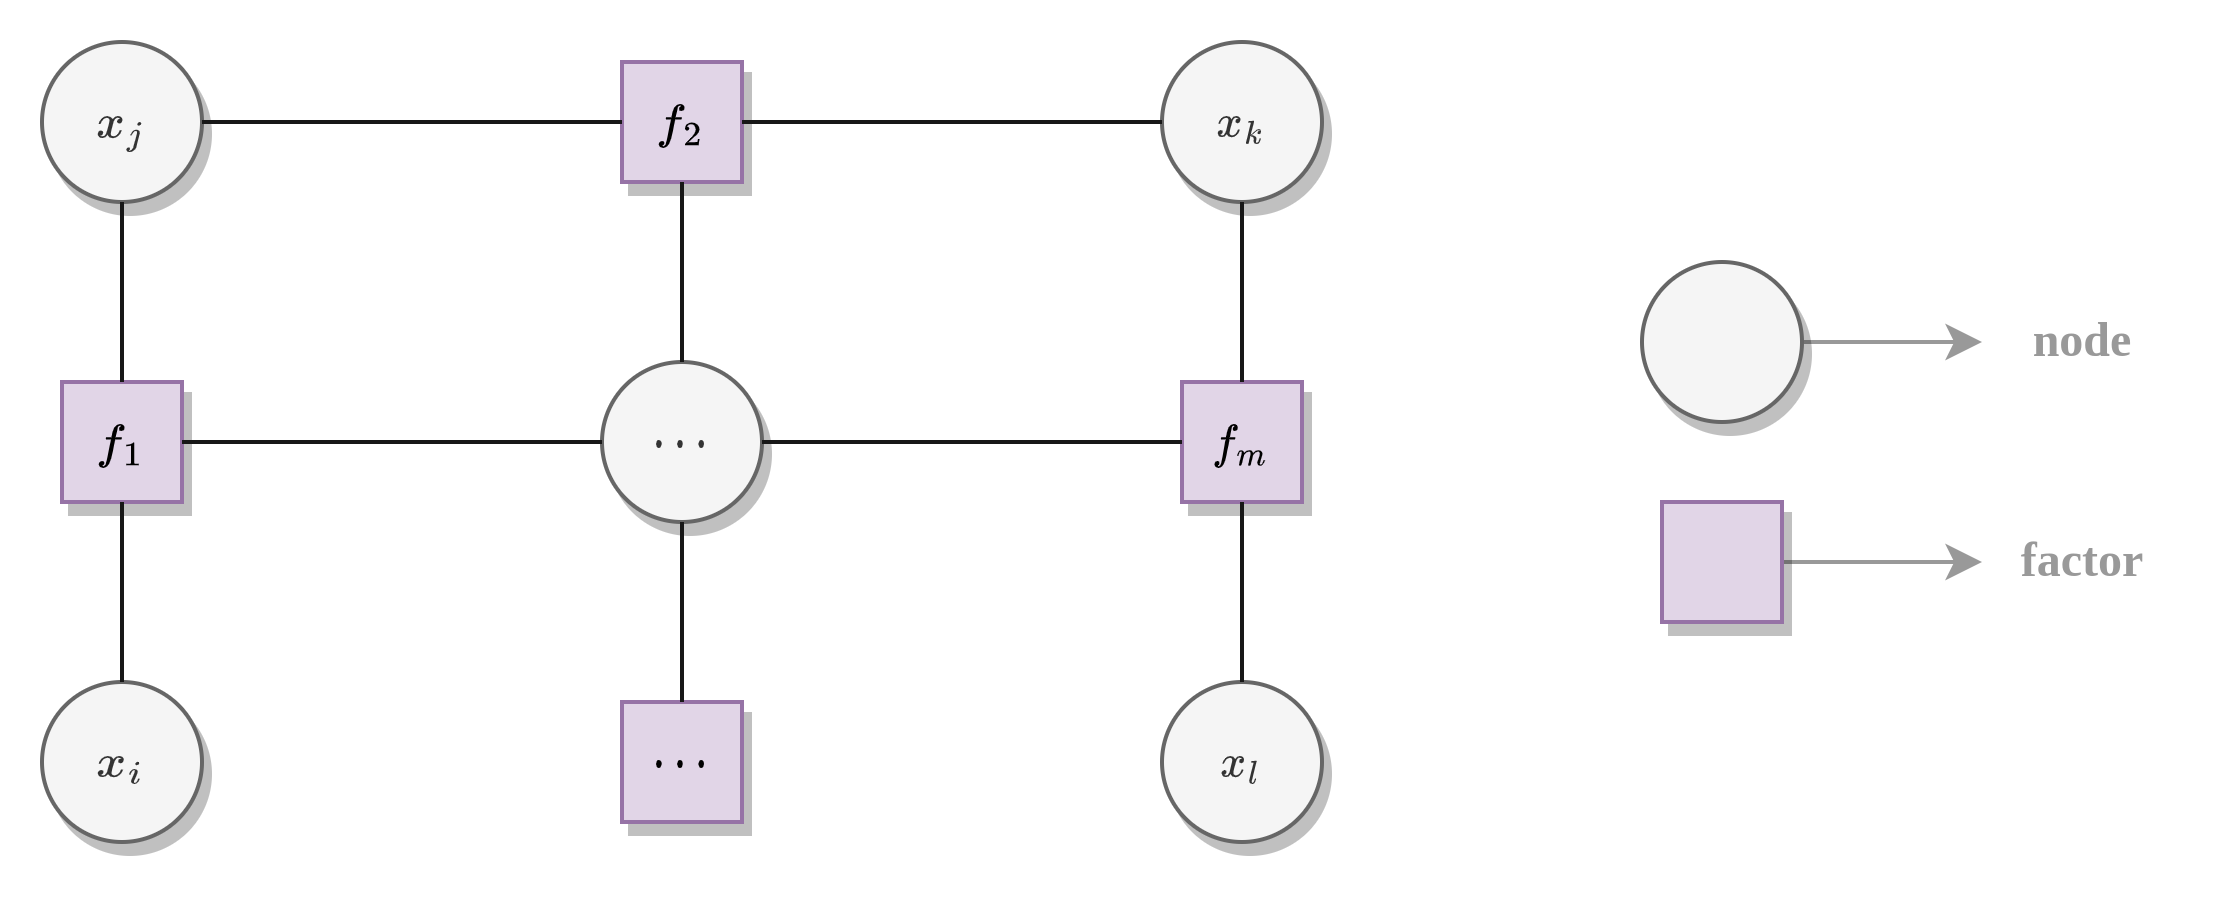
\includegraphics[width=0.5\linewidth]{img/factor_exam.png}
    \caption{\normf{因子图优化的图表示}}
    \label{fig:factor_graphs}
  \end{figure}
}

对于图优化问题的求解,目前已有许多优秀的开源框架,如Ceres\cite{agarwal2012ceres}、$g^2o$\cite{grisetti2011g2o}、GTSAM\cite{dellaert2012factor}、SE-
Sync\cite{rosen2020certifiably}。本文在处理图优化问题时使用Ceres图优化框架, 因为相较于其他开源框架,Ceres在易用性、可扩展性、安全性以及计算效率等方面都比较突出\cite{juric2021comparison}。
